\documentclass[../main.tex]{subfiles}
\graphicspath{../images/results/plots/}

\begin{document}

\chapter{Results}

\section{Results of simple geometry simulations}

\subsection{Cube}

\subsection{Triangles}

\subsection{Chamfered}

\section{Results of femoral components}



\subsection{Displacement analysis}

For the displacement analysis of the femoral component, statistics on the surface mesh of the simulation results were computed. From this graph,  

Figure \ref{fig:disp_ridges} shows the distribution of the surface nodal displacements of the femoral component. The utility of this graph is to visualize easily how the displacements of each result are distributed. We see that the distribution is asymmetrical and it does not resemble a normal distribution. From the other graphs, it can also be observed that the hyperbolic tangent variation within volume fraction group creates slight differences in the distribution of nodal displacements, although it seems only to occur in some particular cases. Lastly, it can be seen from these graphs that the lower volume fractions of 25\% and 33\% have slightly thicker right-end tails, suggesting that there is a greater number of nodes with high displacement as compared to the other simulations.

\begin{figure}[h!]
  \centering
  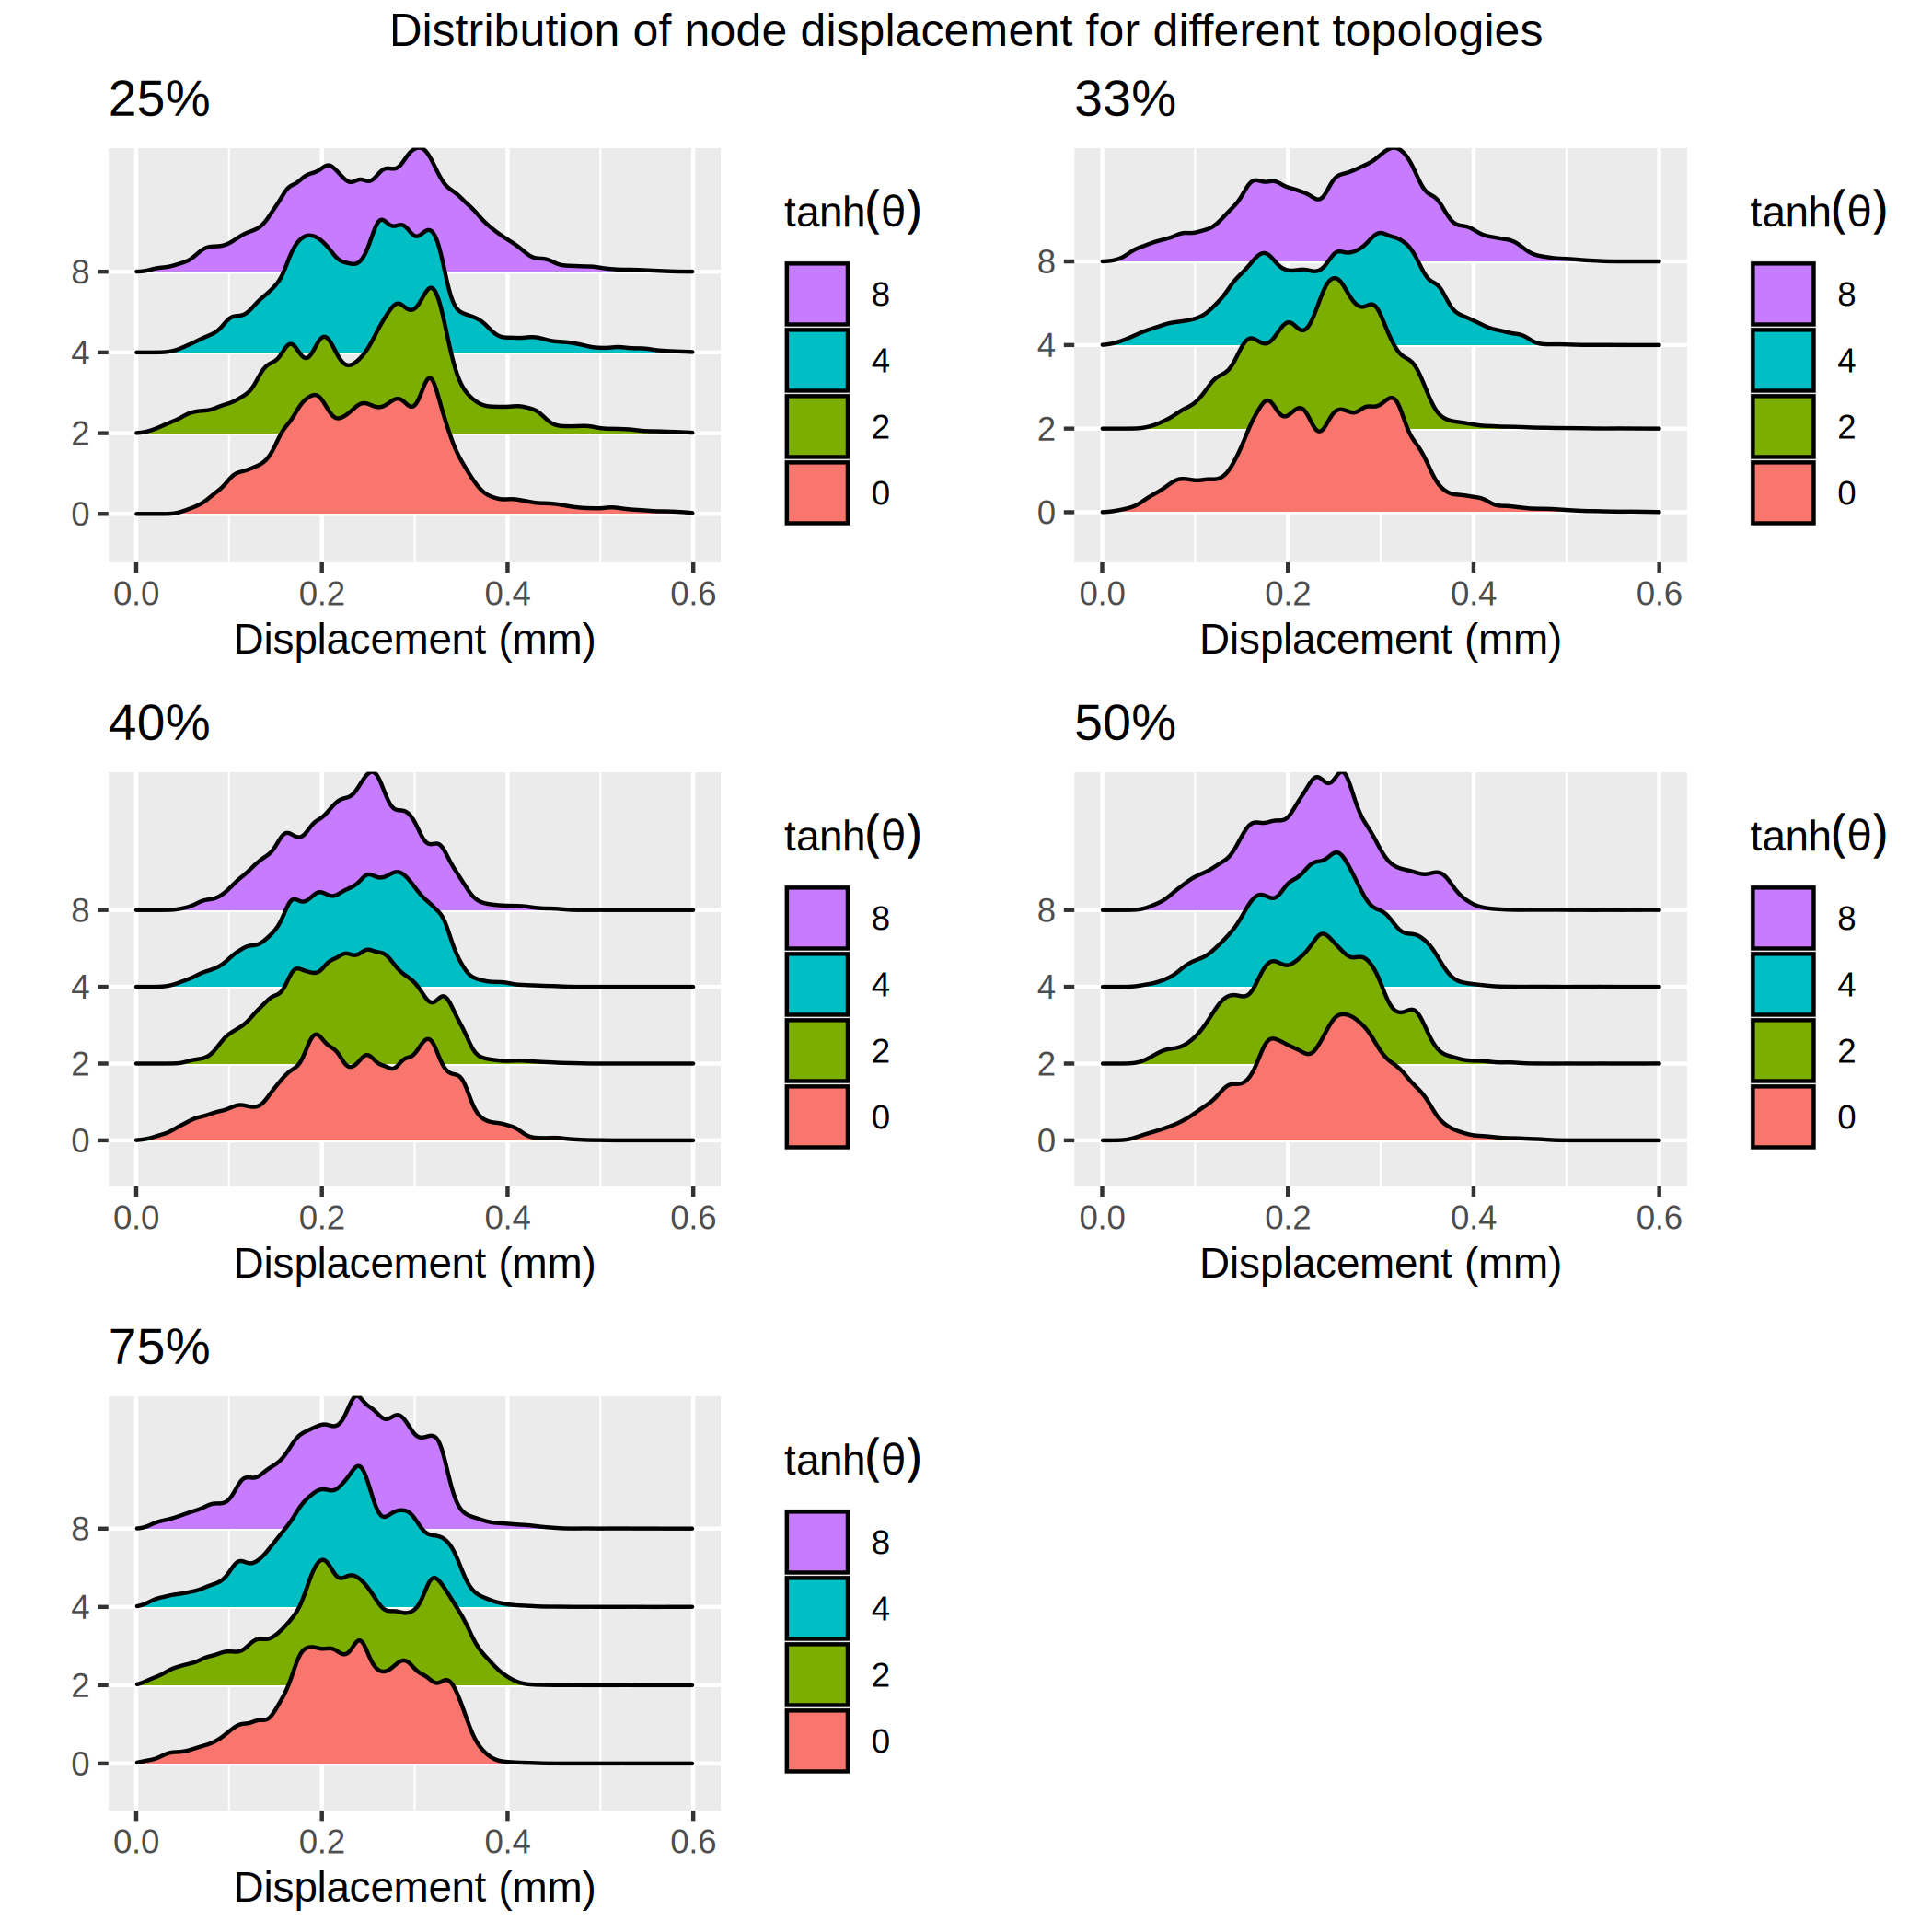
\includegraphics[width=0.9\textwidth]{images/results/plots/femoral/displacement/disp_density_ridges.png}
  \caption{Density distribution of nodal displacements, grouped by volume fraction and hyperbolic tangent angle.}
  \label{fig:disp_ridges}
\end{figure}

This trend can be more easily visualized by computing the average nodal deformation for each case. The left graph of Figure \ref{fig:disp_averages} shows the average nodal deformation, where each column corresponds to a simulation result and each color represents a particular volume fraction group. It is clear from this graphs that the 25\% and 33\% volume fraction results exhibit a slightly larger average deformation compared to the rest of the simulations. This is more clearly show in the right figure, which shows the average deformation for each volume fraction group as a whole. Nevertheless, this difference between average nodal deformation could still be attributed to the numerical uncertainty due to voxelization, as it had been previously established that the numerical errors of the simulation could account up to a variability of 0.01mm.


\begin{figure}[h!]
  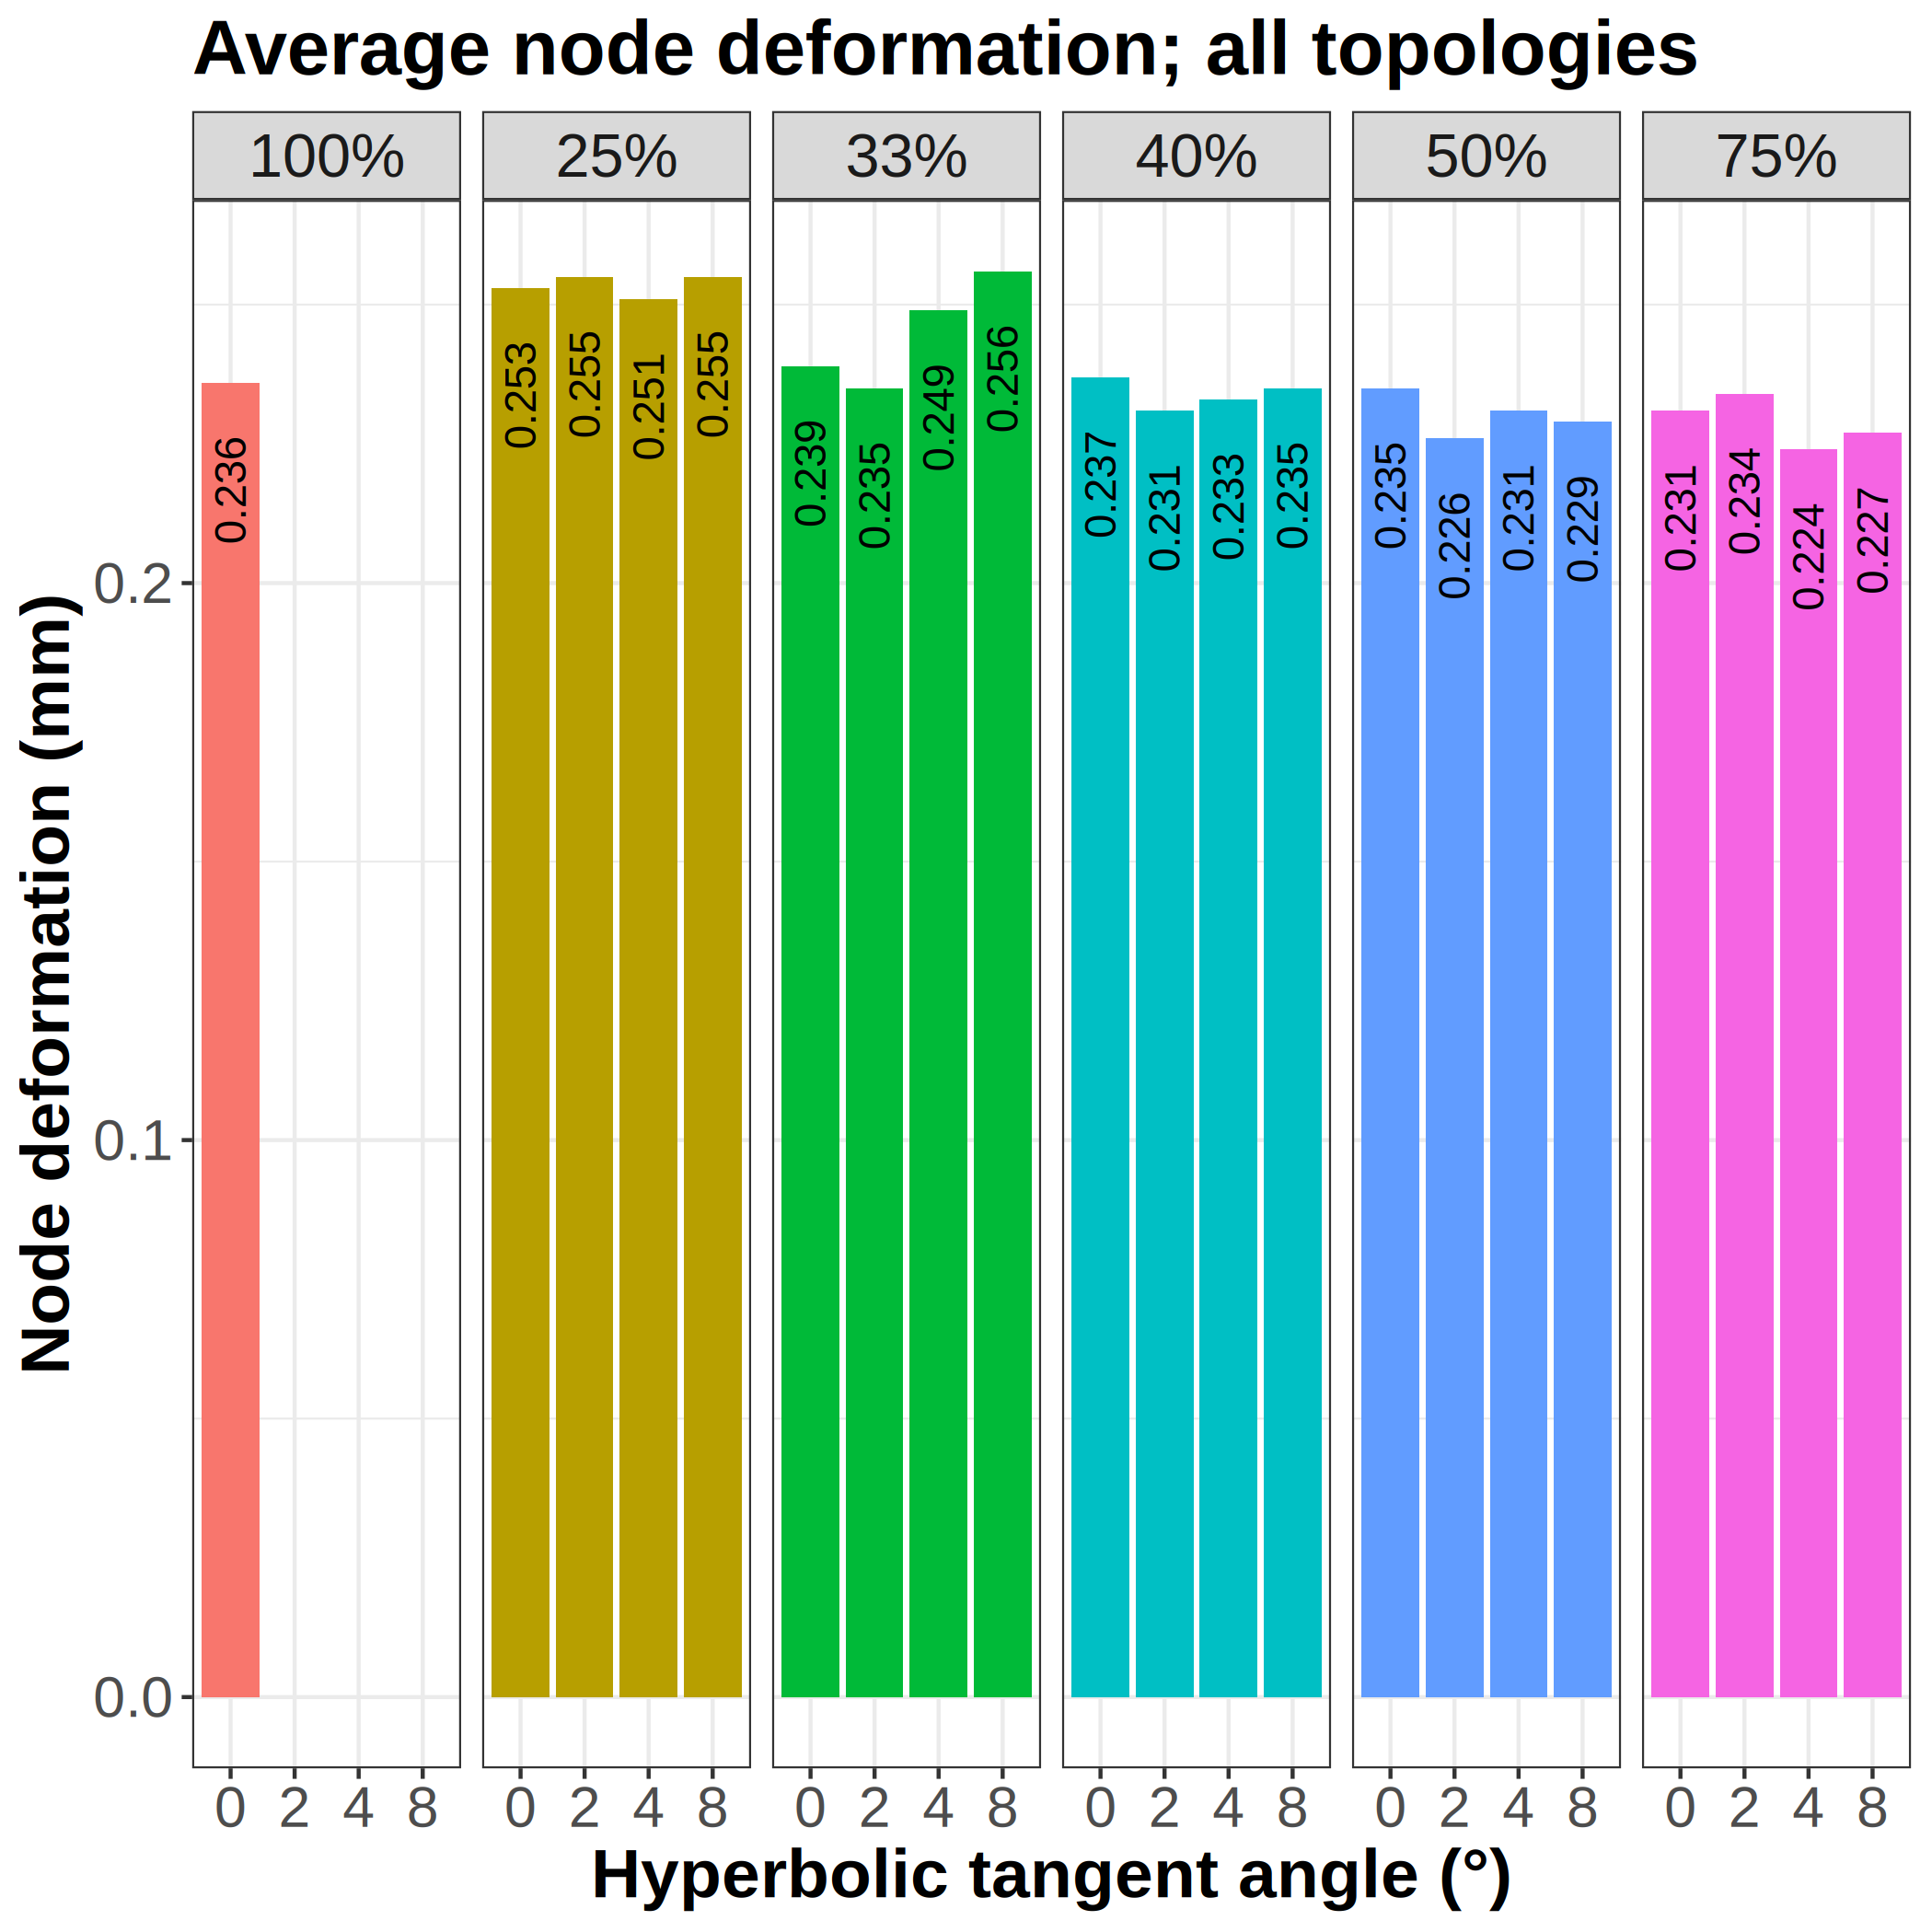
\includegraphics[width=0.45\textwidth]{images/results/plots/femoral/displacement/femoral_average.png}
  \hfill 
  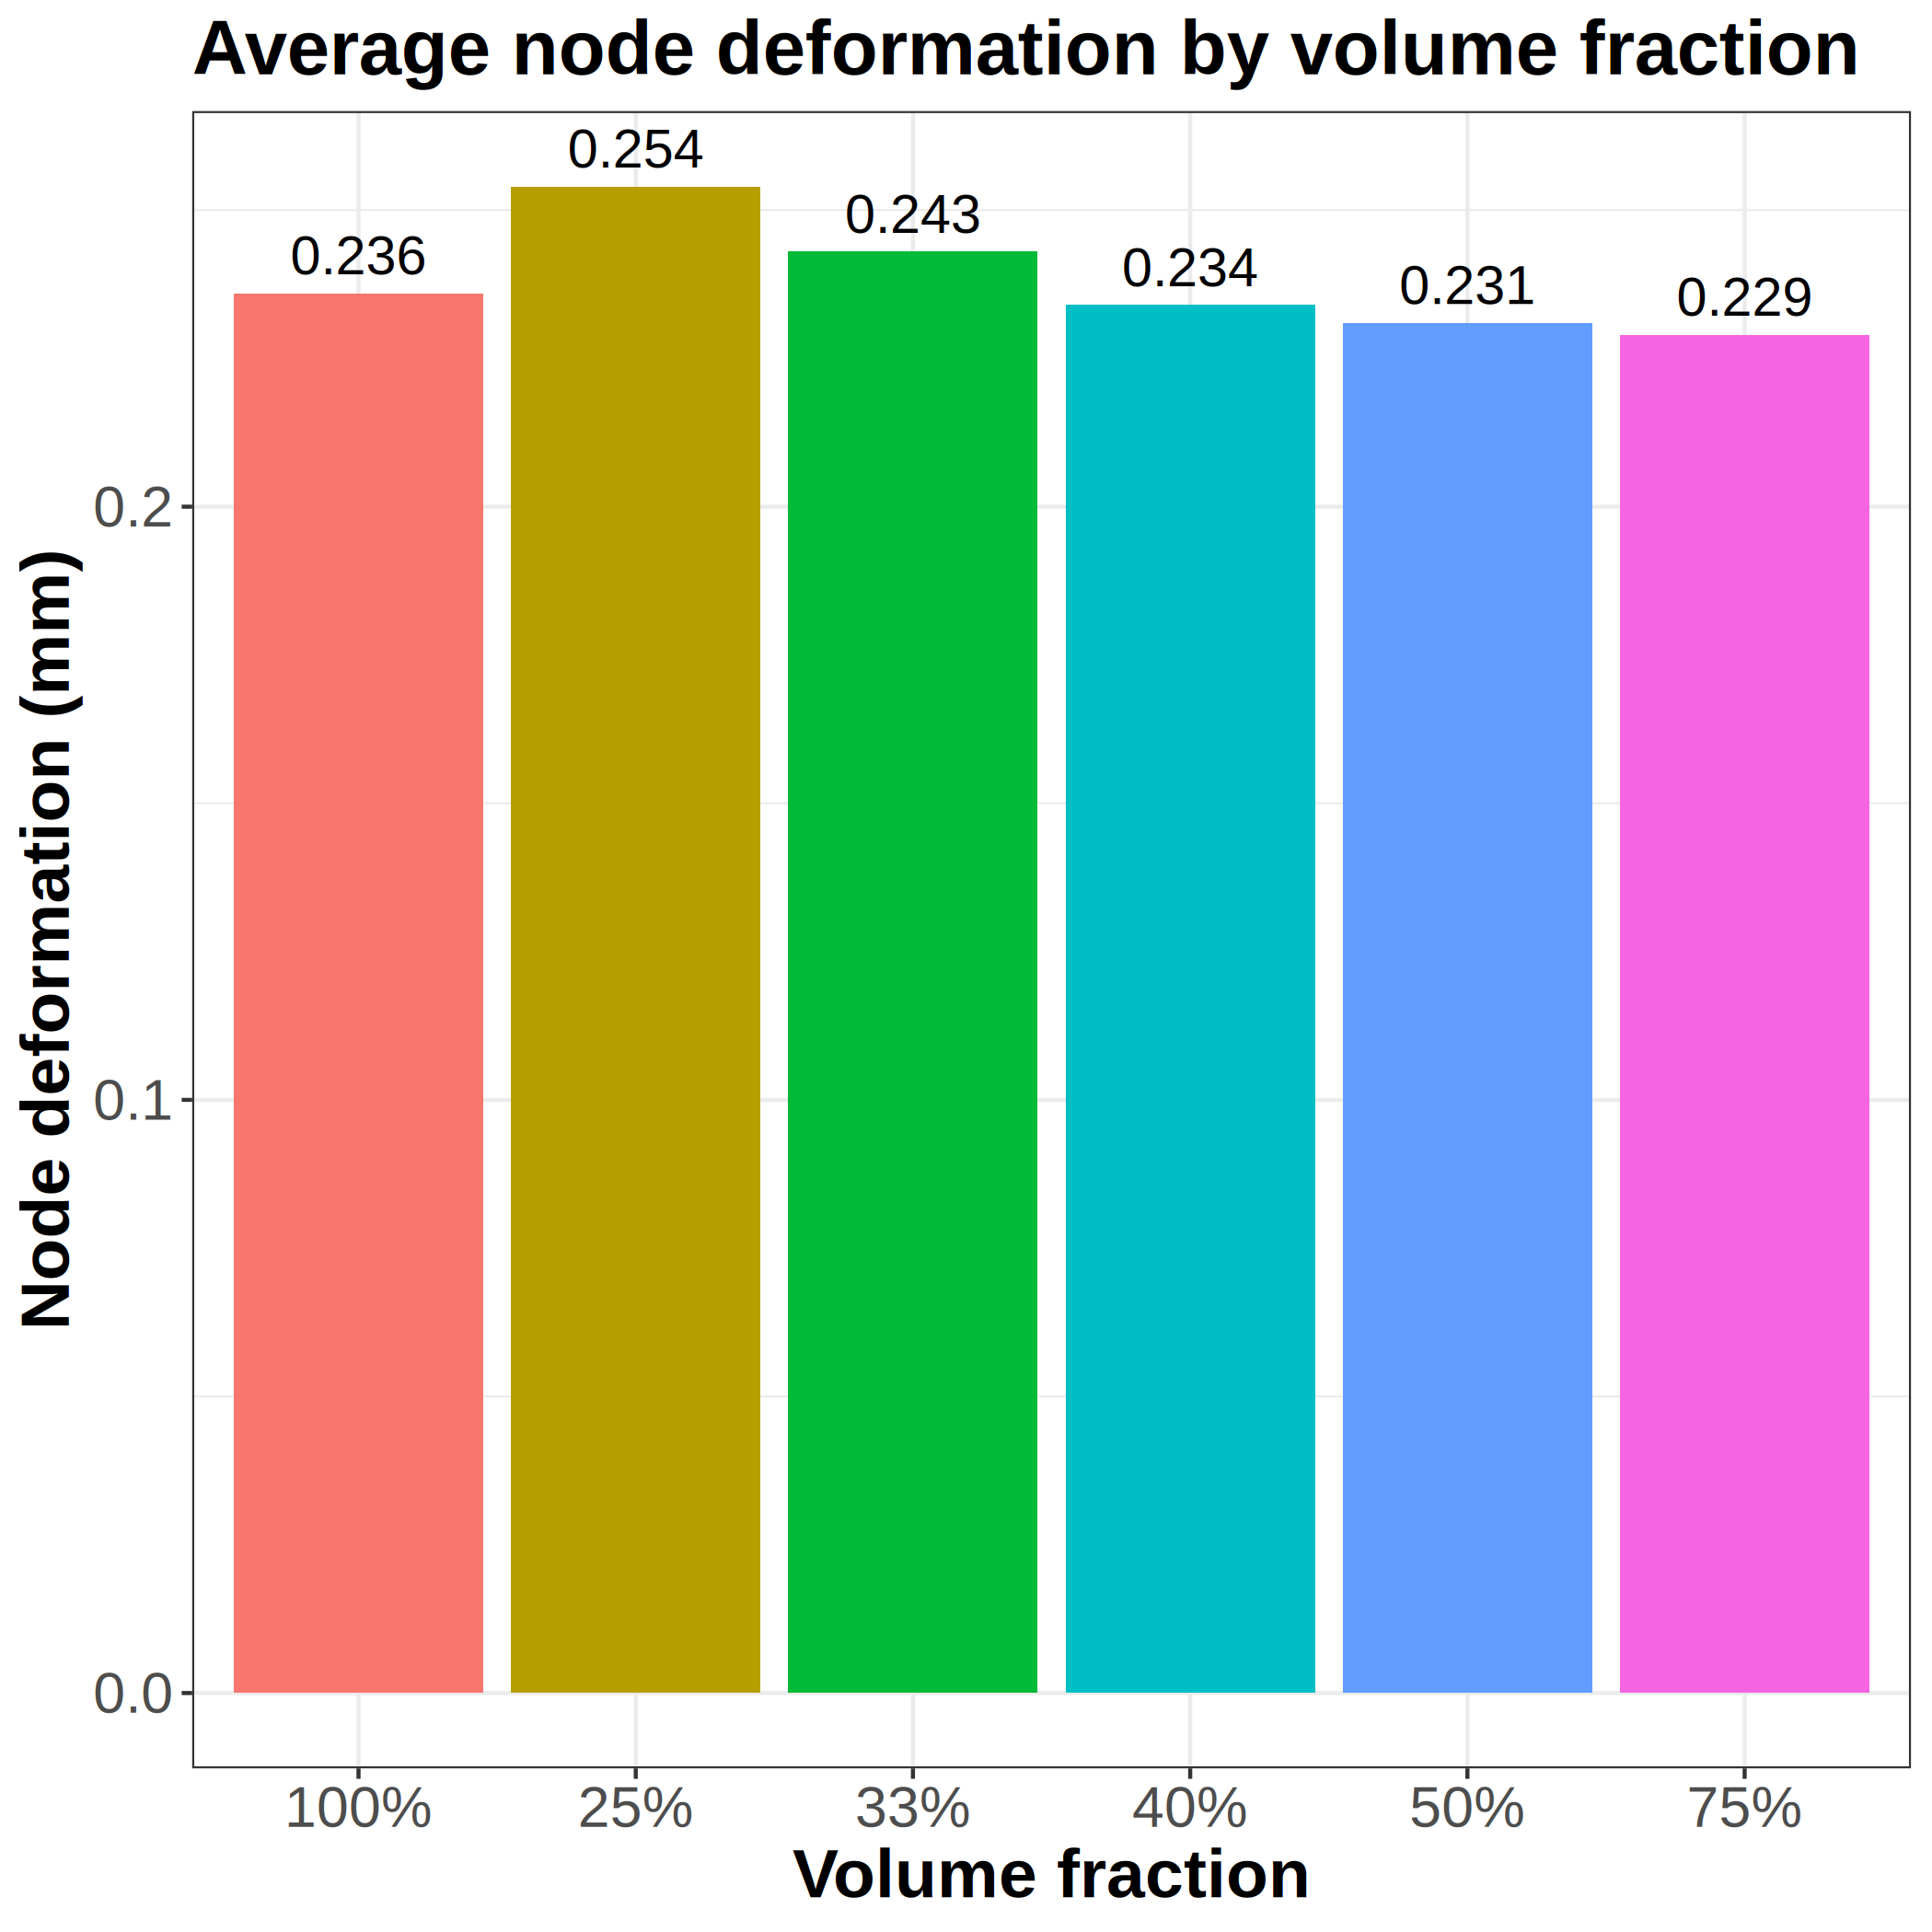
\includegraphics[width=0.45\textwidth]{images/results/plots/femoral/displacement/femoral_average_group.png}
  \caption{Average and max nodal displacement for femoral component simulations.}
  \label{fig:disp_averages}
\end{figure}

Next, the maximum nodal displacements of each group were computed. The results are shown in Figure \ref{fig:disp_max_bad}. There are three results that show excessive deformation at a few nodes. Additionally, it was noticed during the simulation that some voxels exhibited abnormal behavior, and deformed in a non-physical manner. This is showcased in Figure \ref{fig:bad_voxel}, where one voxel has merged into a neighboring one. Therefore, it is highly suspected that the results for these geometries show faulty node displacements caused by a bug or anomaly in the finite element calculation. To determine whether these excessive deformations are significant, the deformation were binned in bins of 0.1 mm. The result of this operation is shown in  Figure \ref{fig:disp_bins}.

\begin{figure}[h!]
  \centering
  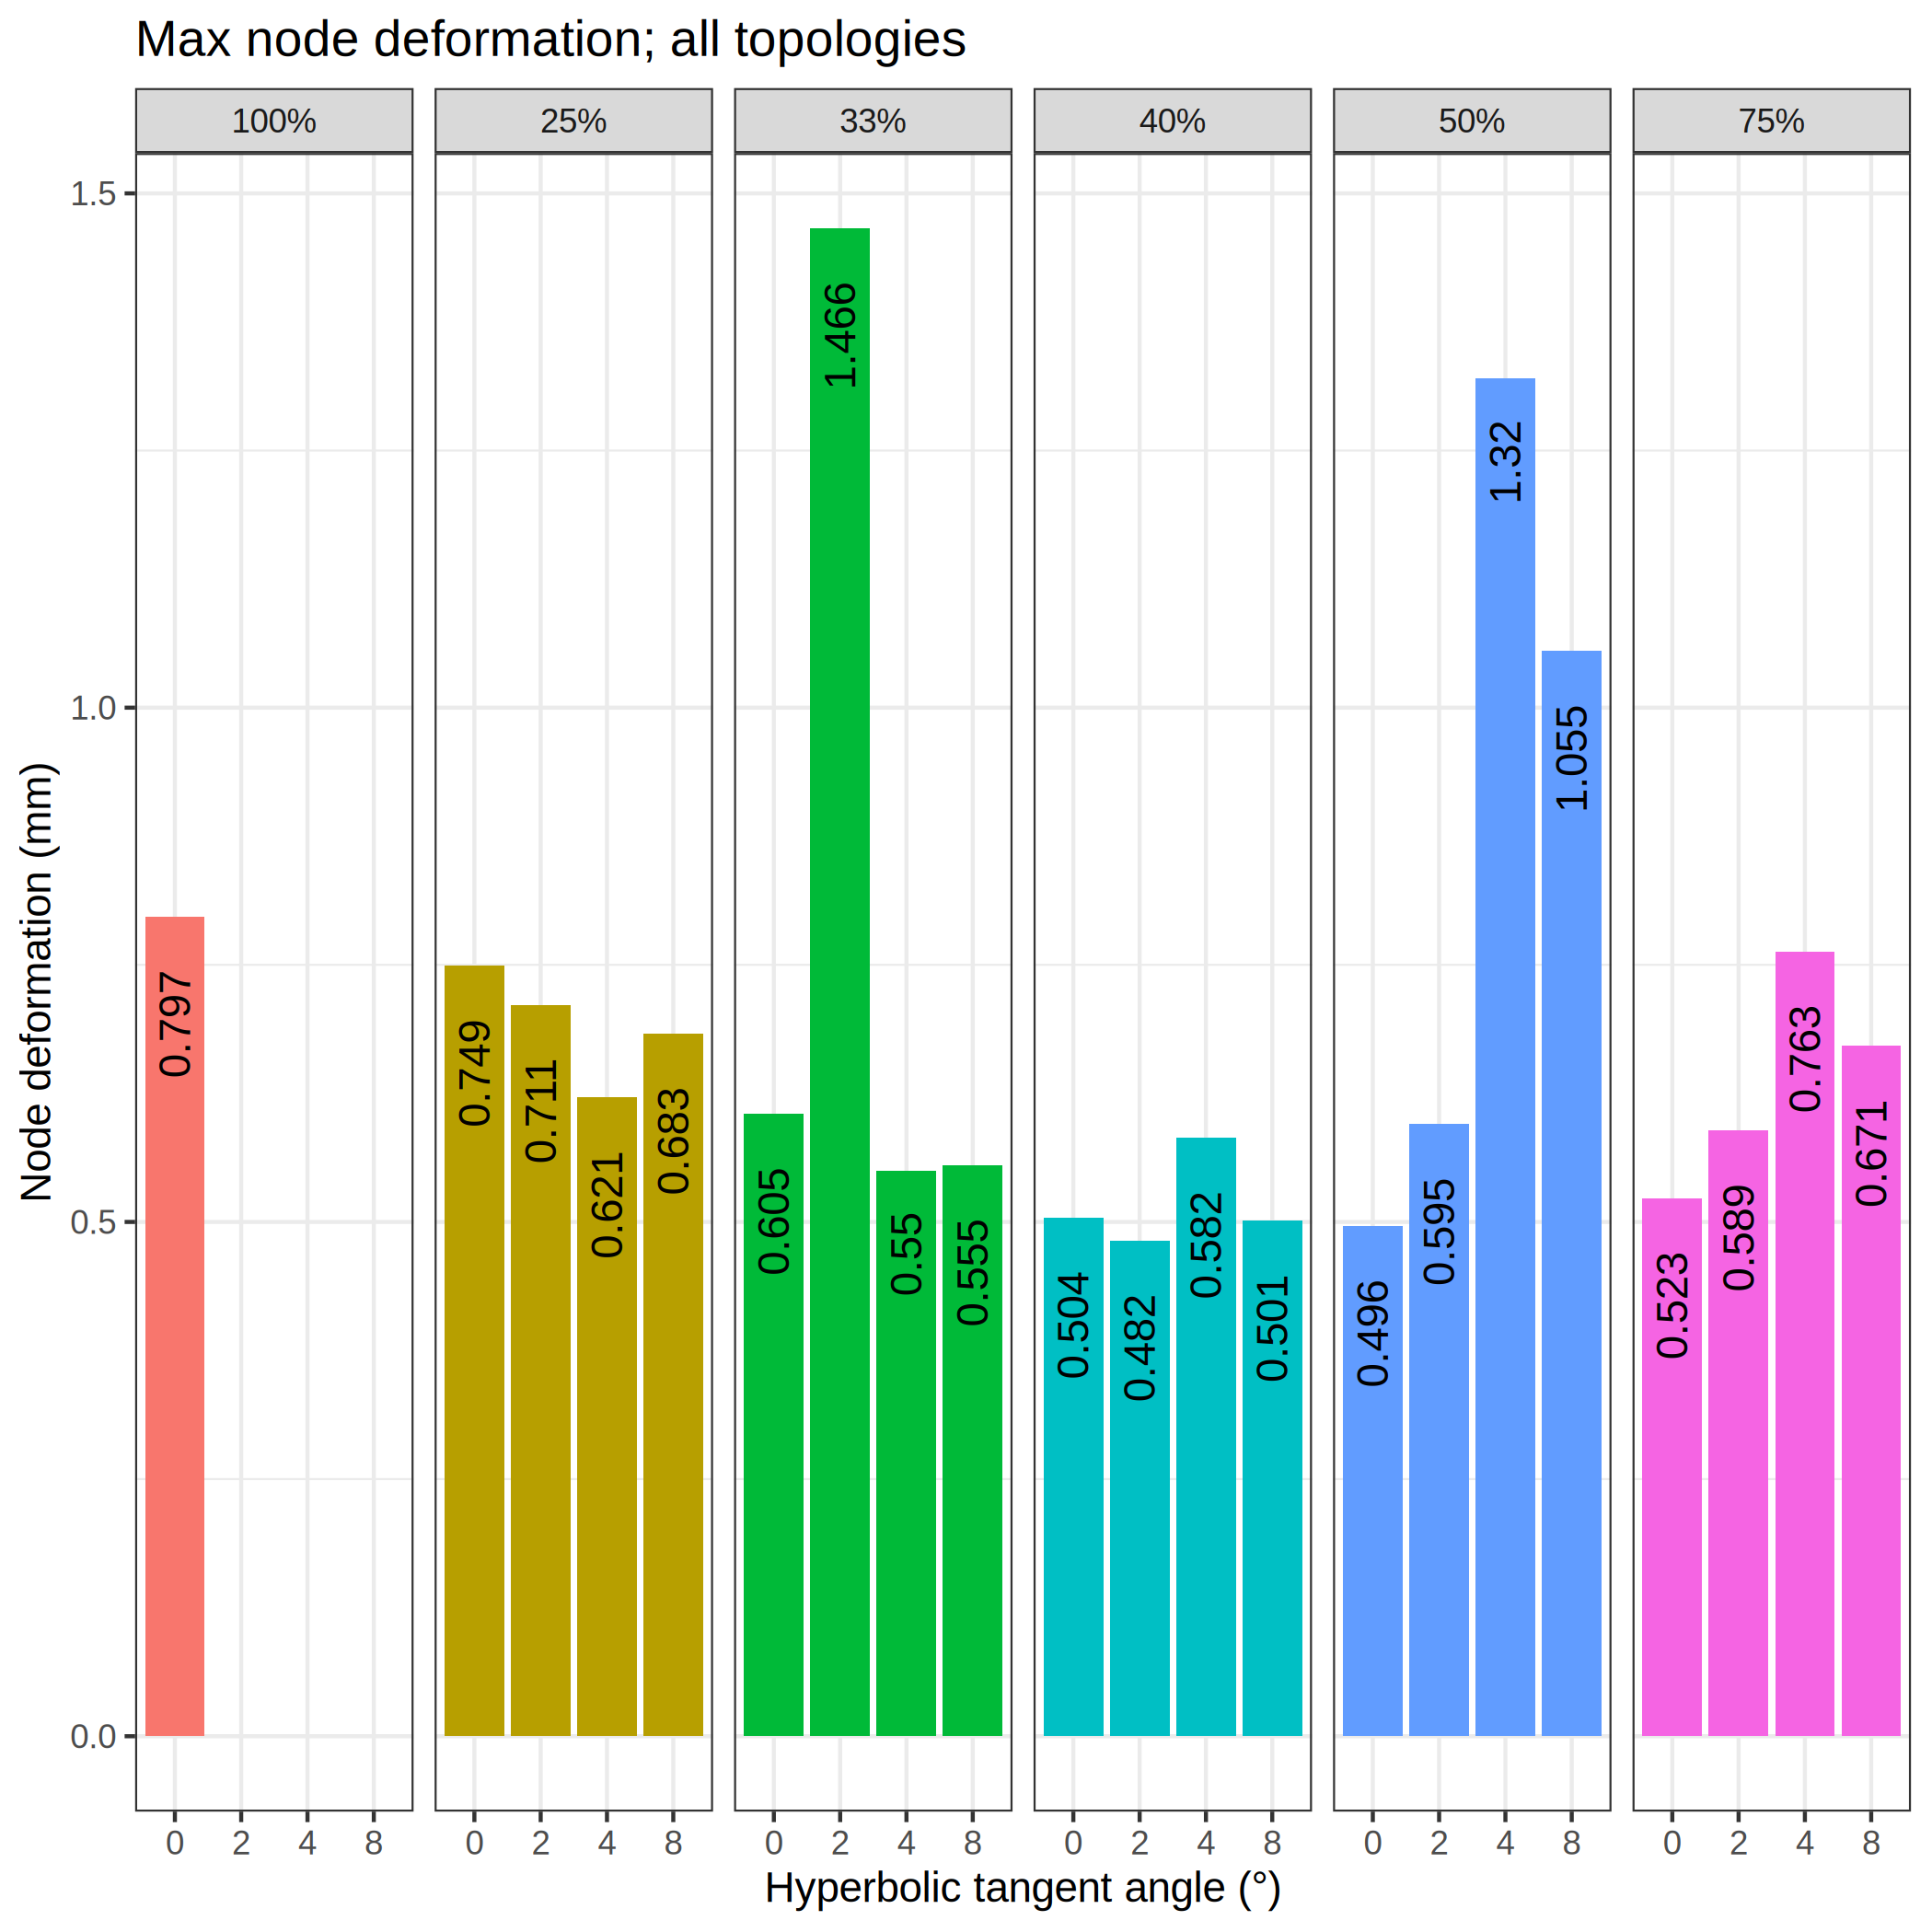
\includegraphics[width=0.6\textwidth]{images/results/plots/femoral/displacement/femoral_max_bad.png}
  \caption{Maximum nodal displacements for the femoral component simulations. Notice that there are three topologies that show an excessive maximal displacement. These displacements are very likely to be outliers, and further analysis was done to understand their nature.}
  \label{fig:disp_max_bad}
\end{figure}

\begin{figure}[h!]
  \centering
  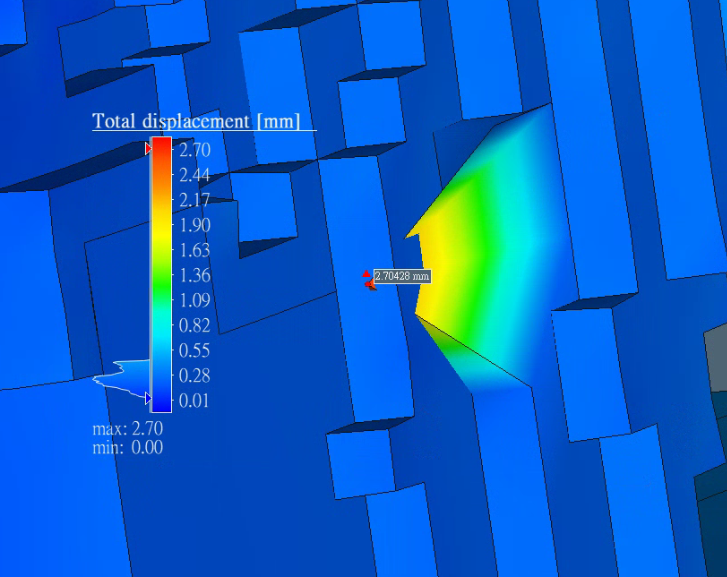
\includegraphics[width=0.6\textwidth]{images/bad_voxel.png}
  \caption{Screenshot of abnormal voxel behavior from simulation result. The voxel seems to be deformed and merging inside the structure itself. Luckily, only a handful of voxels of these sort exist, with the rest of the geometry showing much more sensible results.}
  \label{fig:bad_voxel}
\end{figure}

Figure \ref{fig:disp_bins} shows that there are some ranges of deformation that do not contain any nodes, meaning that there are discontinuities in the nodal deformations. This behavior is clearly non-physical, and suggests that these offending nodes should be discarded. To discard them, all nodes further away from three standard deviation were deleted from these topologies, and the statistics were recalculated. The graph of the maximum nodal displacements with corrected distributions are shown in Figure \ref{fig:disp_max_correct}. From this corrected figure it can be seen that there is local minima in the maximum nodal deformation for the results of the 40\% volume fraction simulations. Additionally, the differences between groups is much greater than the numerical uncertainty from the variation due to voxelization ( > 0.011 mm), making this result significant. Therefore, we can infer from this data that variation in topology does not result in a big effect on average node deformation, but can have an impact on the maximum node deformation of the resulting structure.

\begin{figure}[h!]
  \centering
  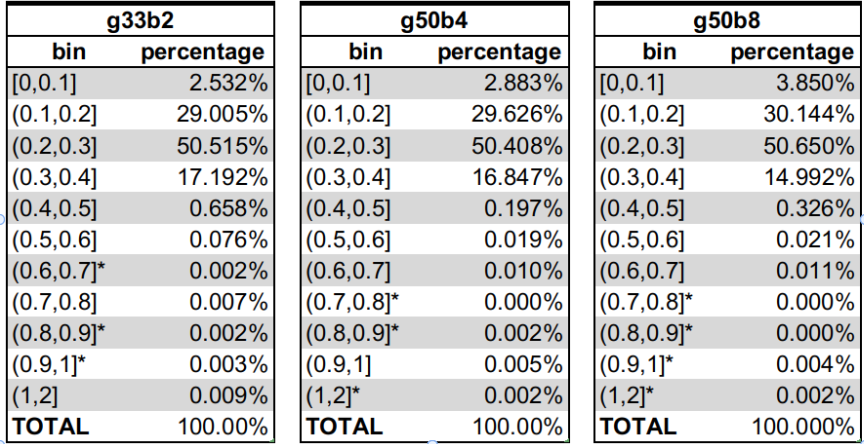
\includegraphics[width=0.75\textwidth]{images/results/plots/femoral/displacement/bins.png}
  \caption{Bins of nodal displacement for suspicious results. The bins labeled with an asterisk have very little to no members, indicating a discontinuous nodal deformation distribution. This is deemed to be non-physical and likely an error with the finite element result.}
  \label{fig:disp_bins}
\end{figure}

\begin{figure}[h!]
  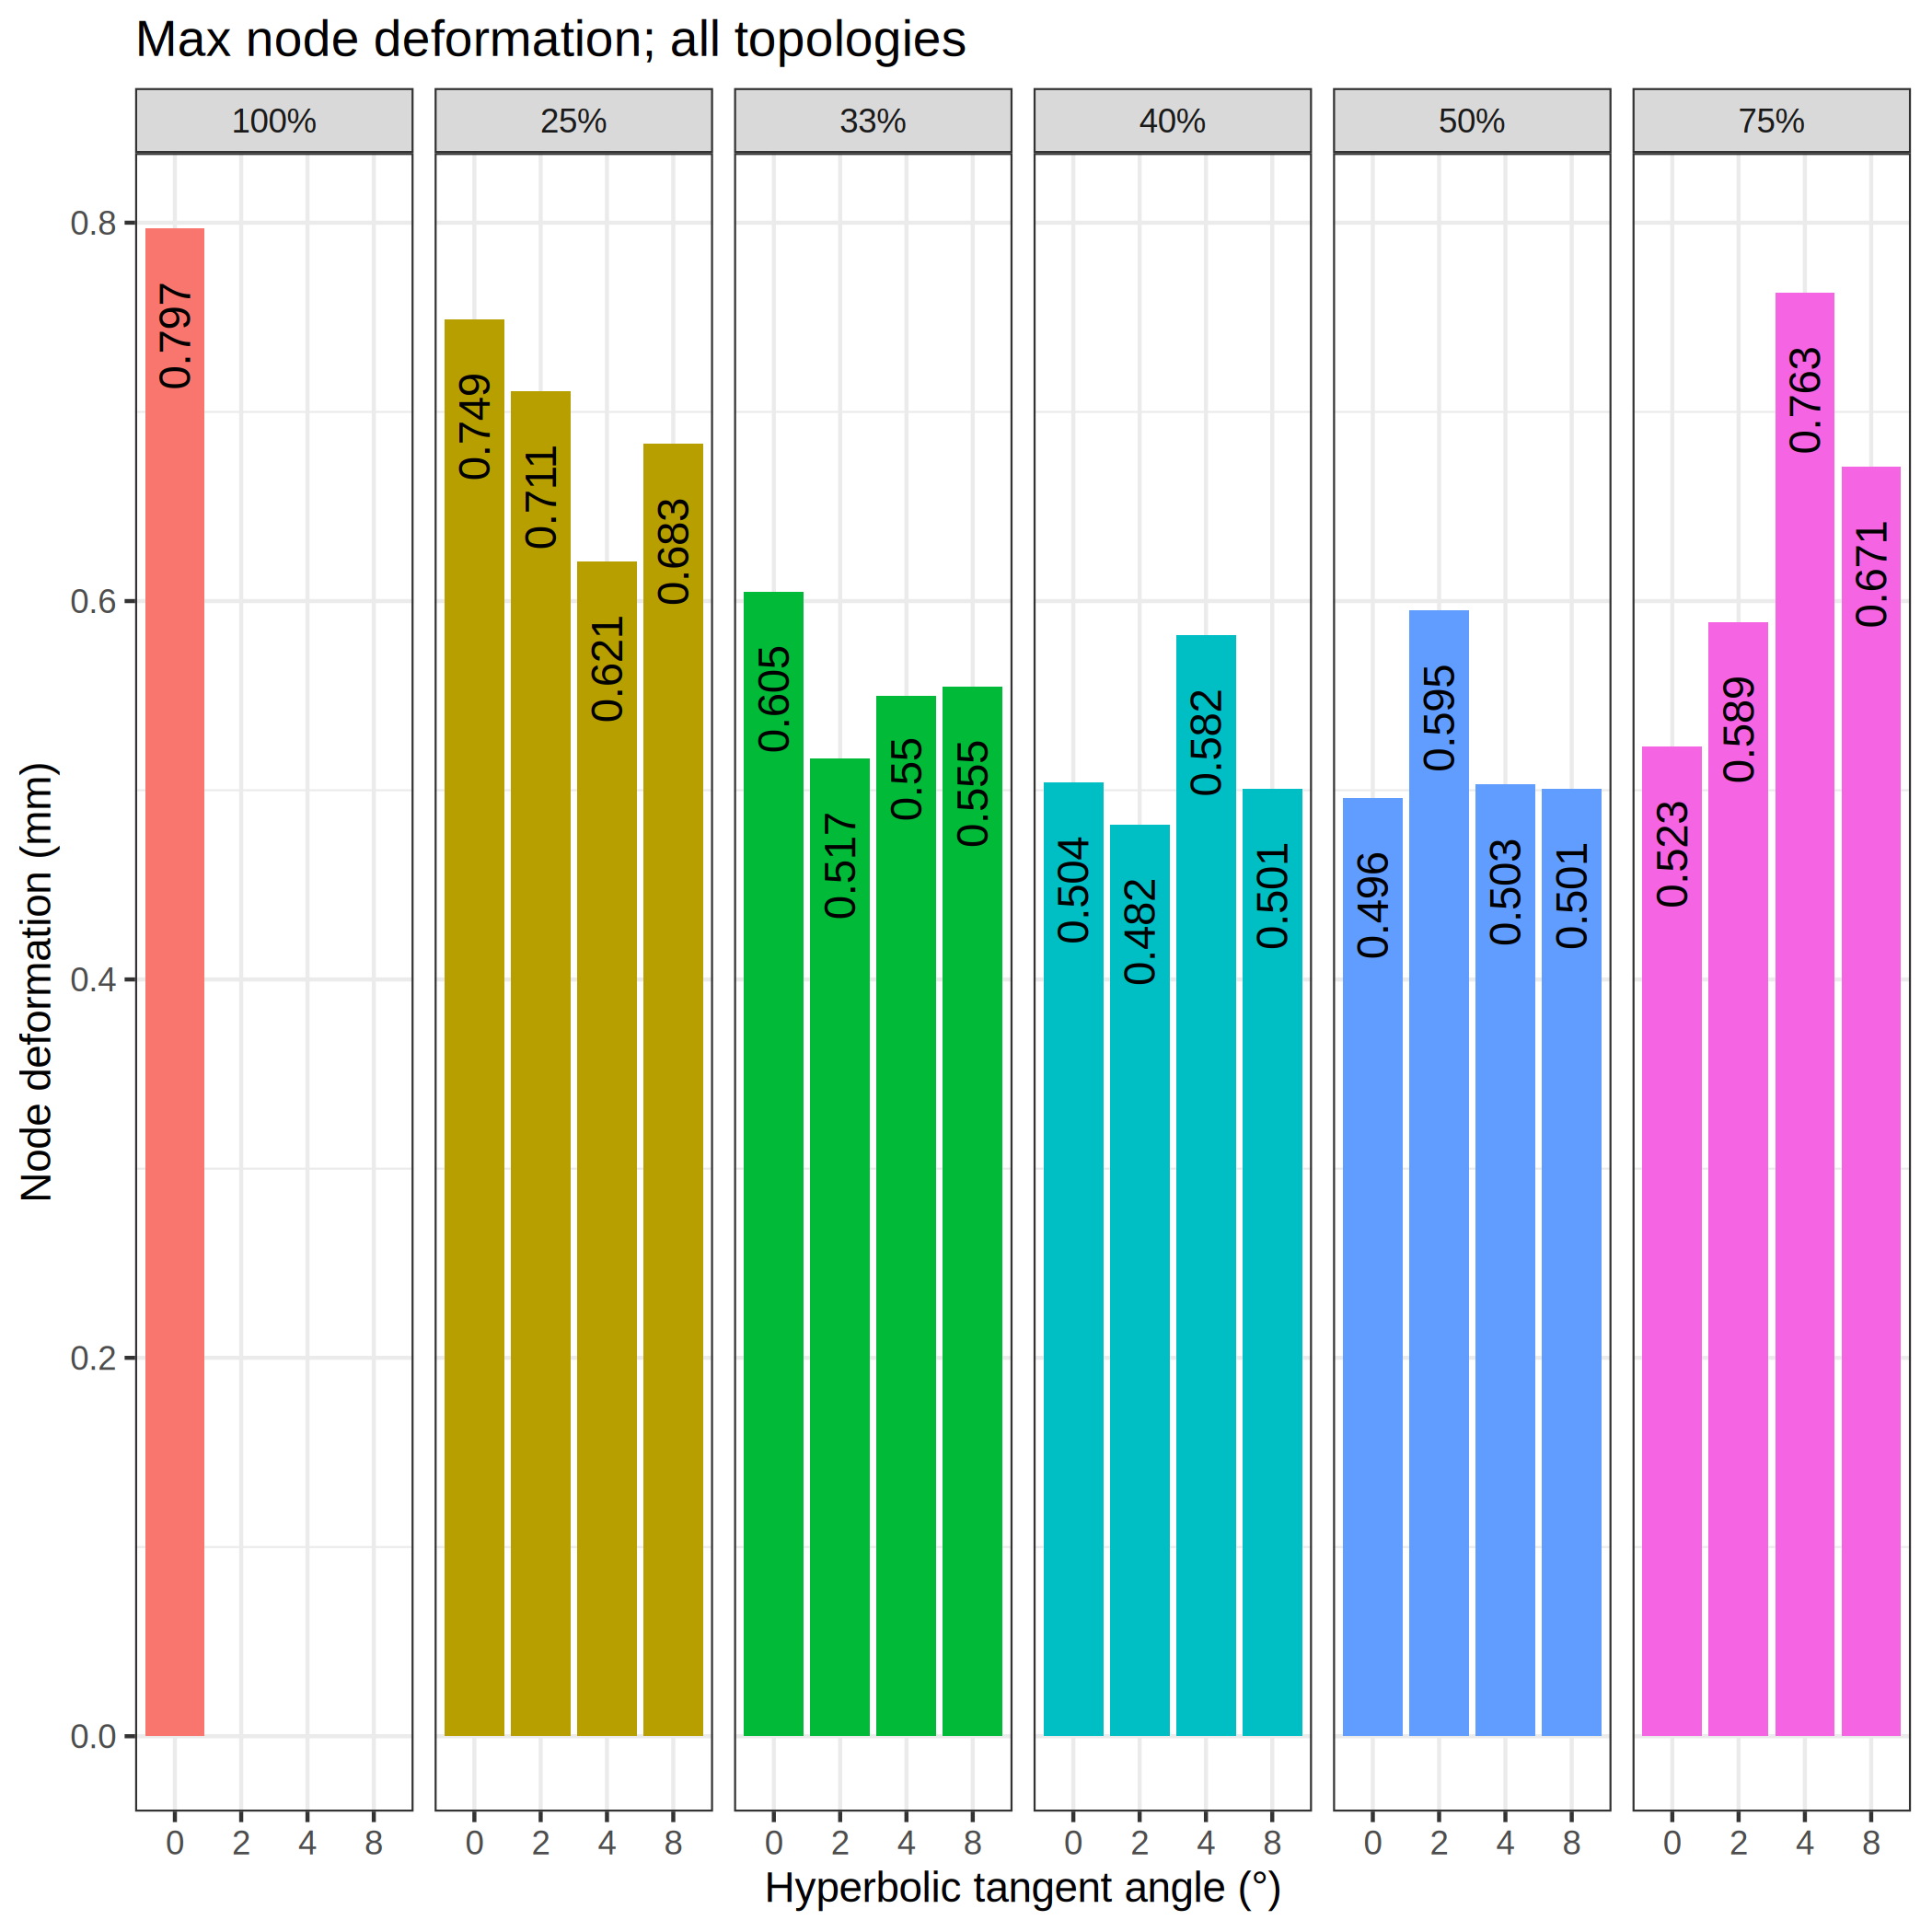
\includegraphics[width=0.45\textwidth]{images/results/plots/femoral/displacement/femoral_max.png}
  \hfill
  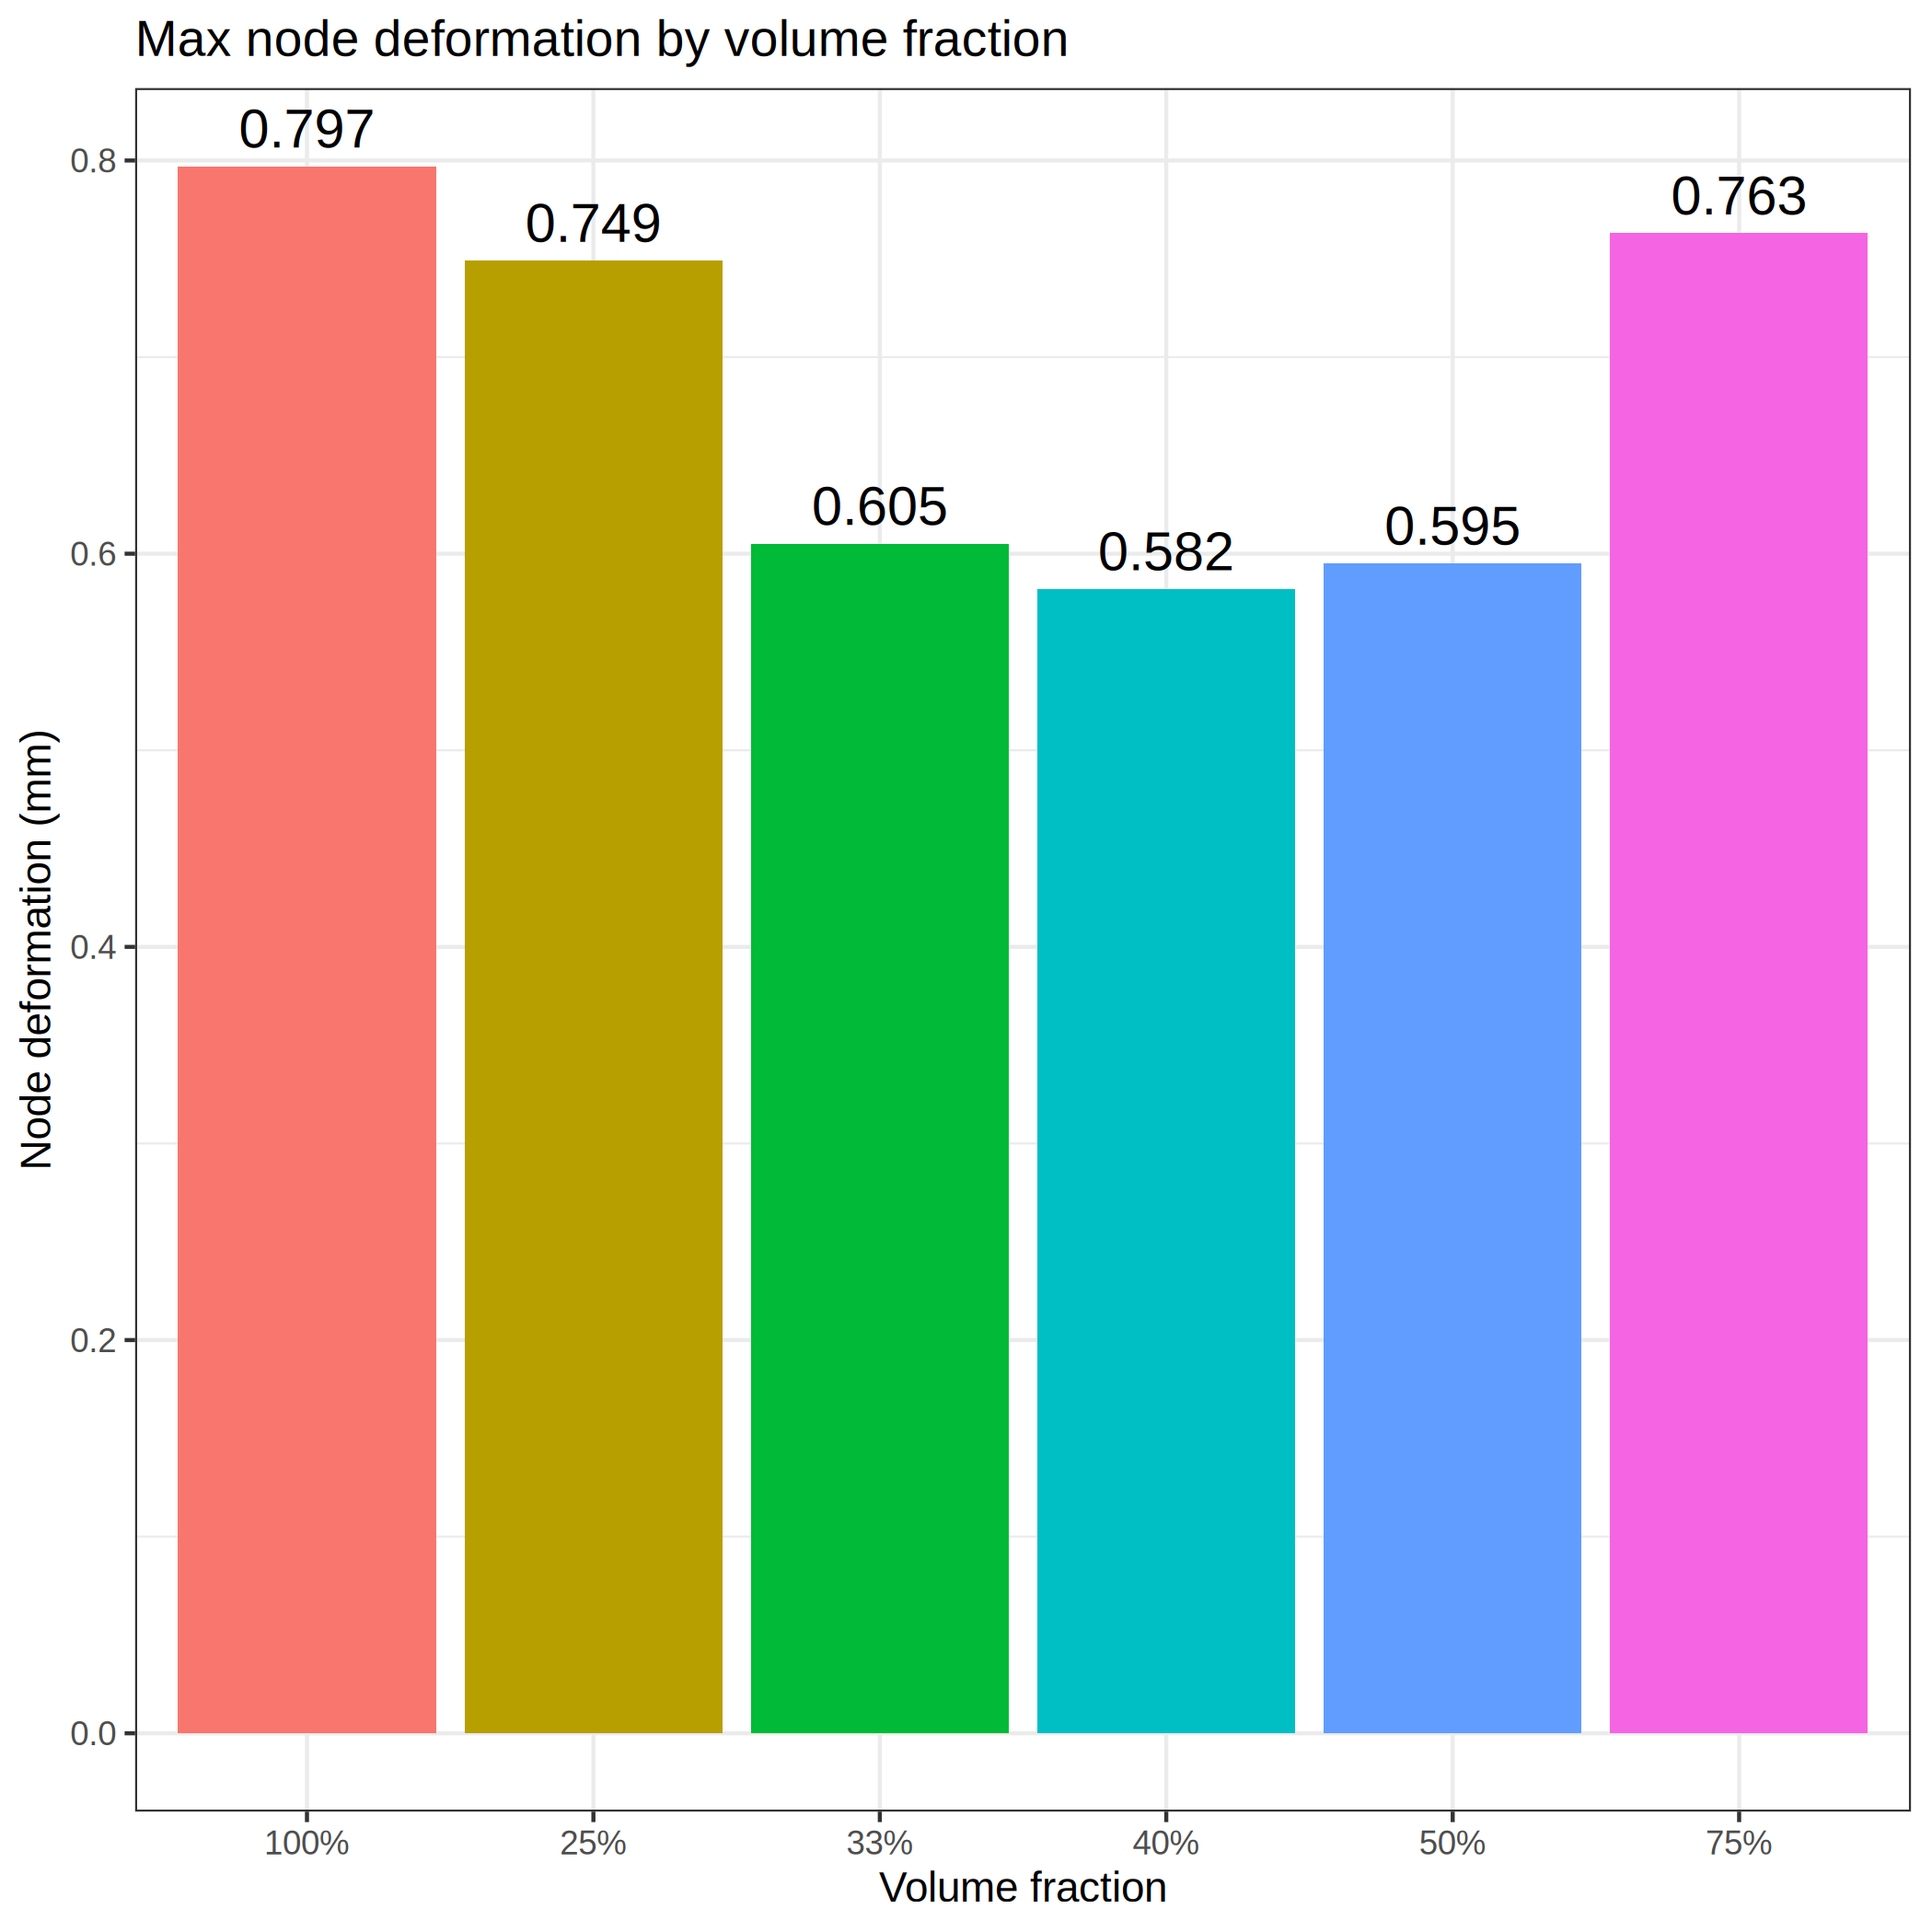
\includegraphics[width=0.45\textwidth]{images/results/plots/femoral/displacement/femoral_max_group.png}
  \caption{Maximum nodal displacement after corrections.}
  \label{fig:disp_max_correct}
\end{figure}

Lastly, all of the following trends can be succintly visualized using a box and whisker plot, shown in Figure \ref{fig:disp_boxwhisker}. From this final plot we can see once more that the average deformation stays constant throughout, but that there is a local minimum in the maximum deformation in the groups with intermediate volume fractions.

\begin{figure}[h!]
  \centering
  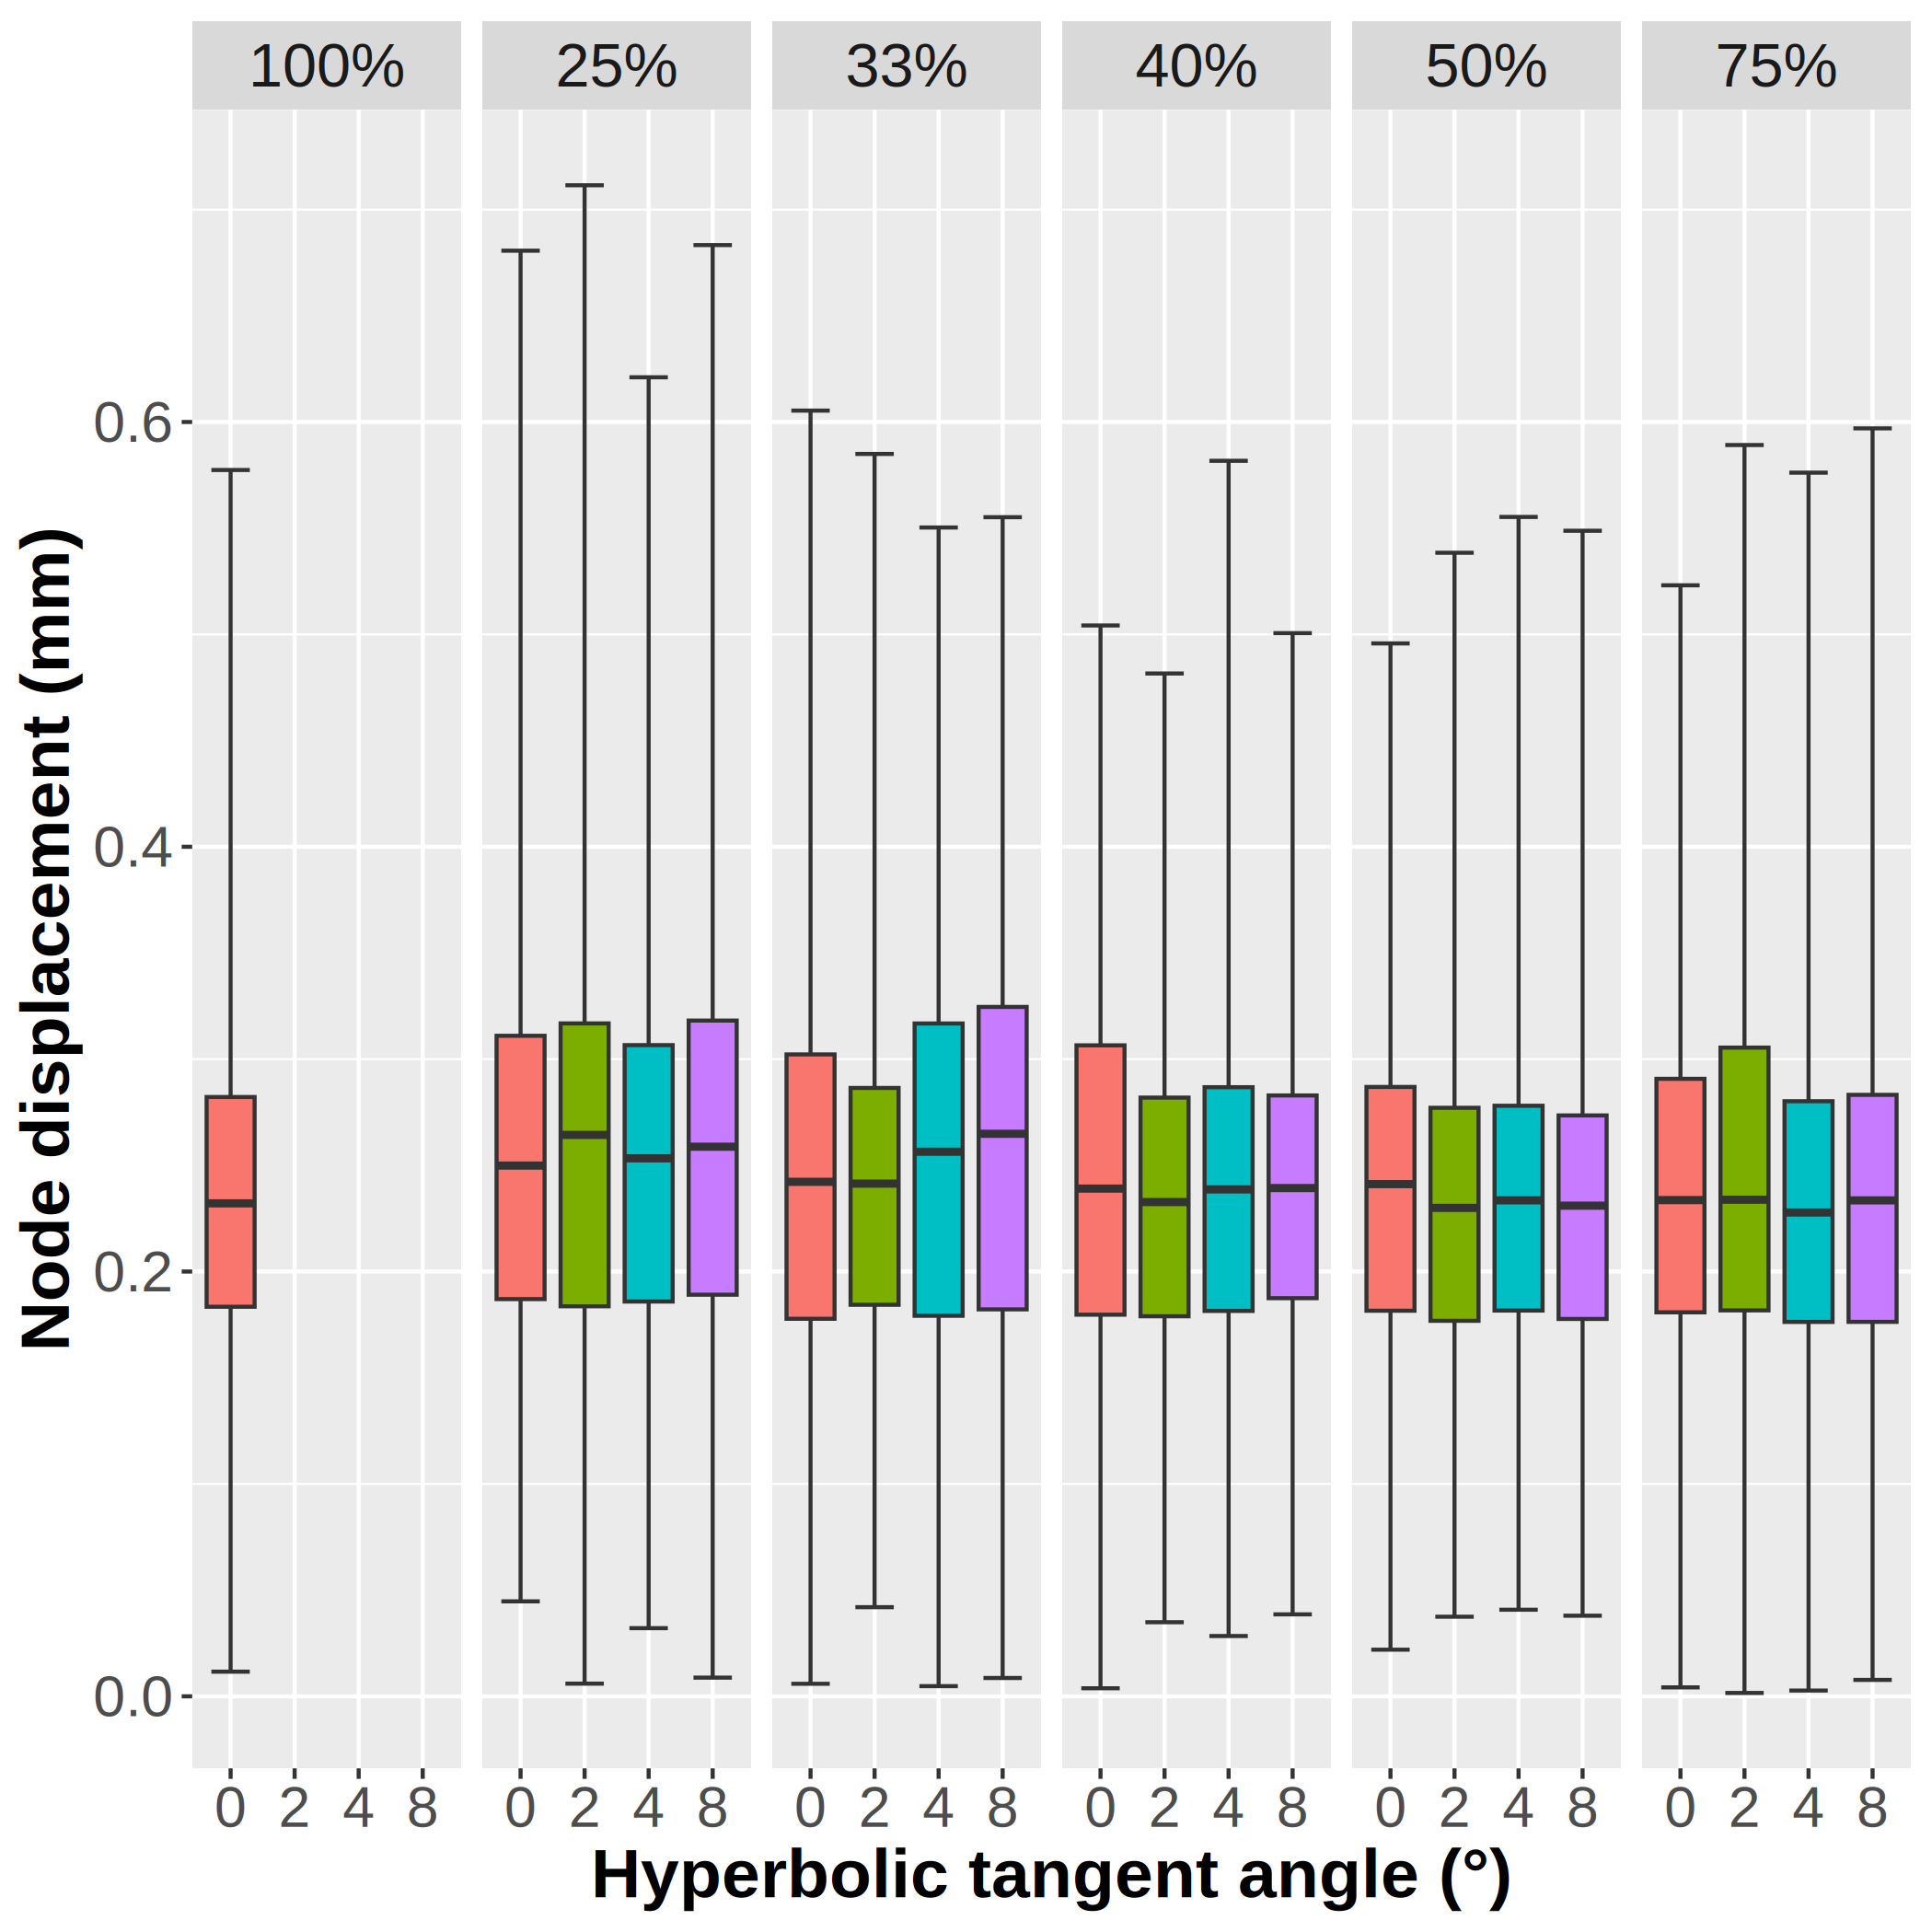
\includegraphics[width=0.6\textwidth]{images/results/plots/femoral/displacement/boxplots.png}
  \caption{Box and whisker plot for femoral displacement of all topologies}
  \label{fig:disp_boxwhisker}
\end{figure}

\clearpage
\subsection{Stress analysis}

To analyze the differences in internal stresses caused by the topologies, we inspect the node stress density distributions. In contrast with the displacement density distribution, there is very little variability between groups. On the other hand, across groups we can see differences in the spread of stress. For example, the stress are most densely concentrated around the peak of the 25\% group compared to the groups with higher volume fractions, such as 50\% and 75\%. This indicates that some groups have smaller standard deviations, with values more closely packed together. This can be confirmed by looking at the statistics in  
Figure \ref{fig:stress_stats}, where we can see slight differences in the standard deviation of topologies.

\begin{figure}[h!]
  \centering
  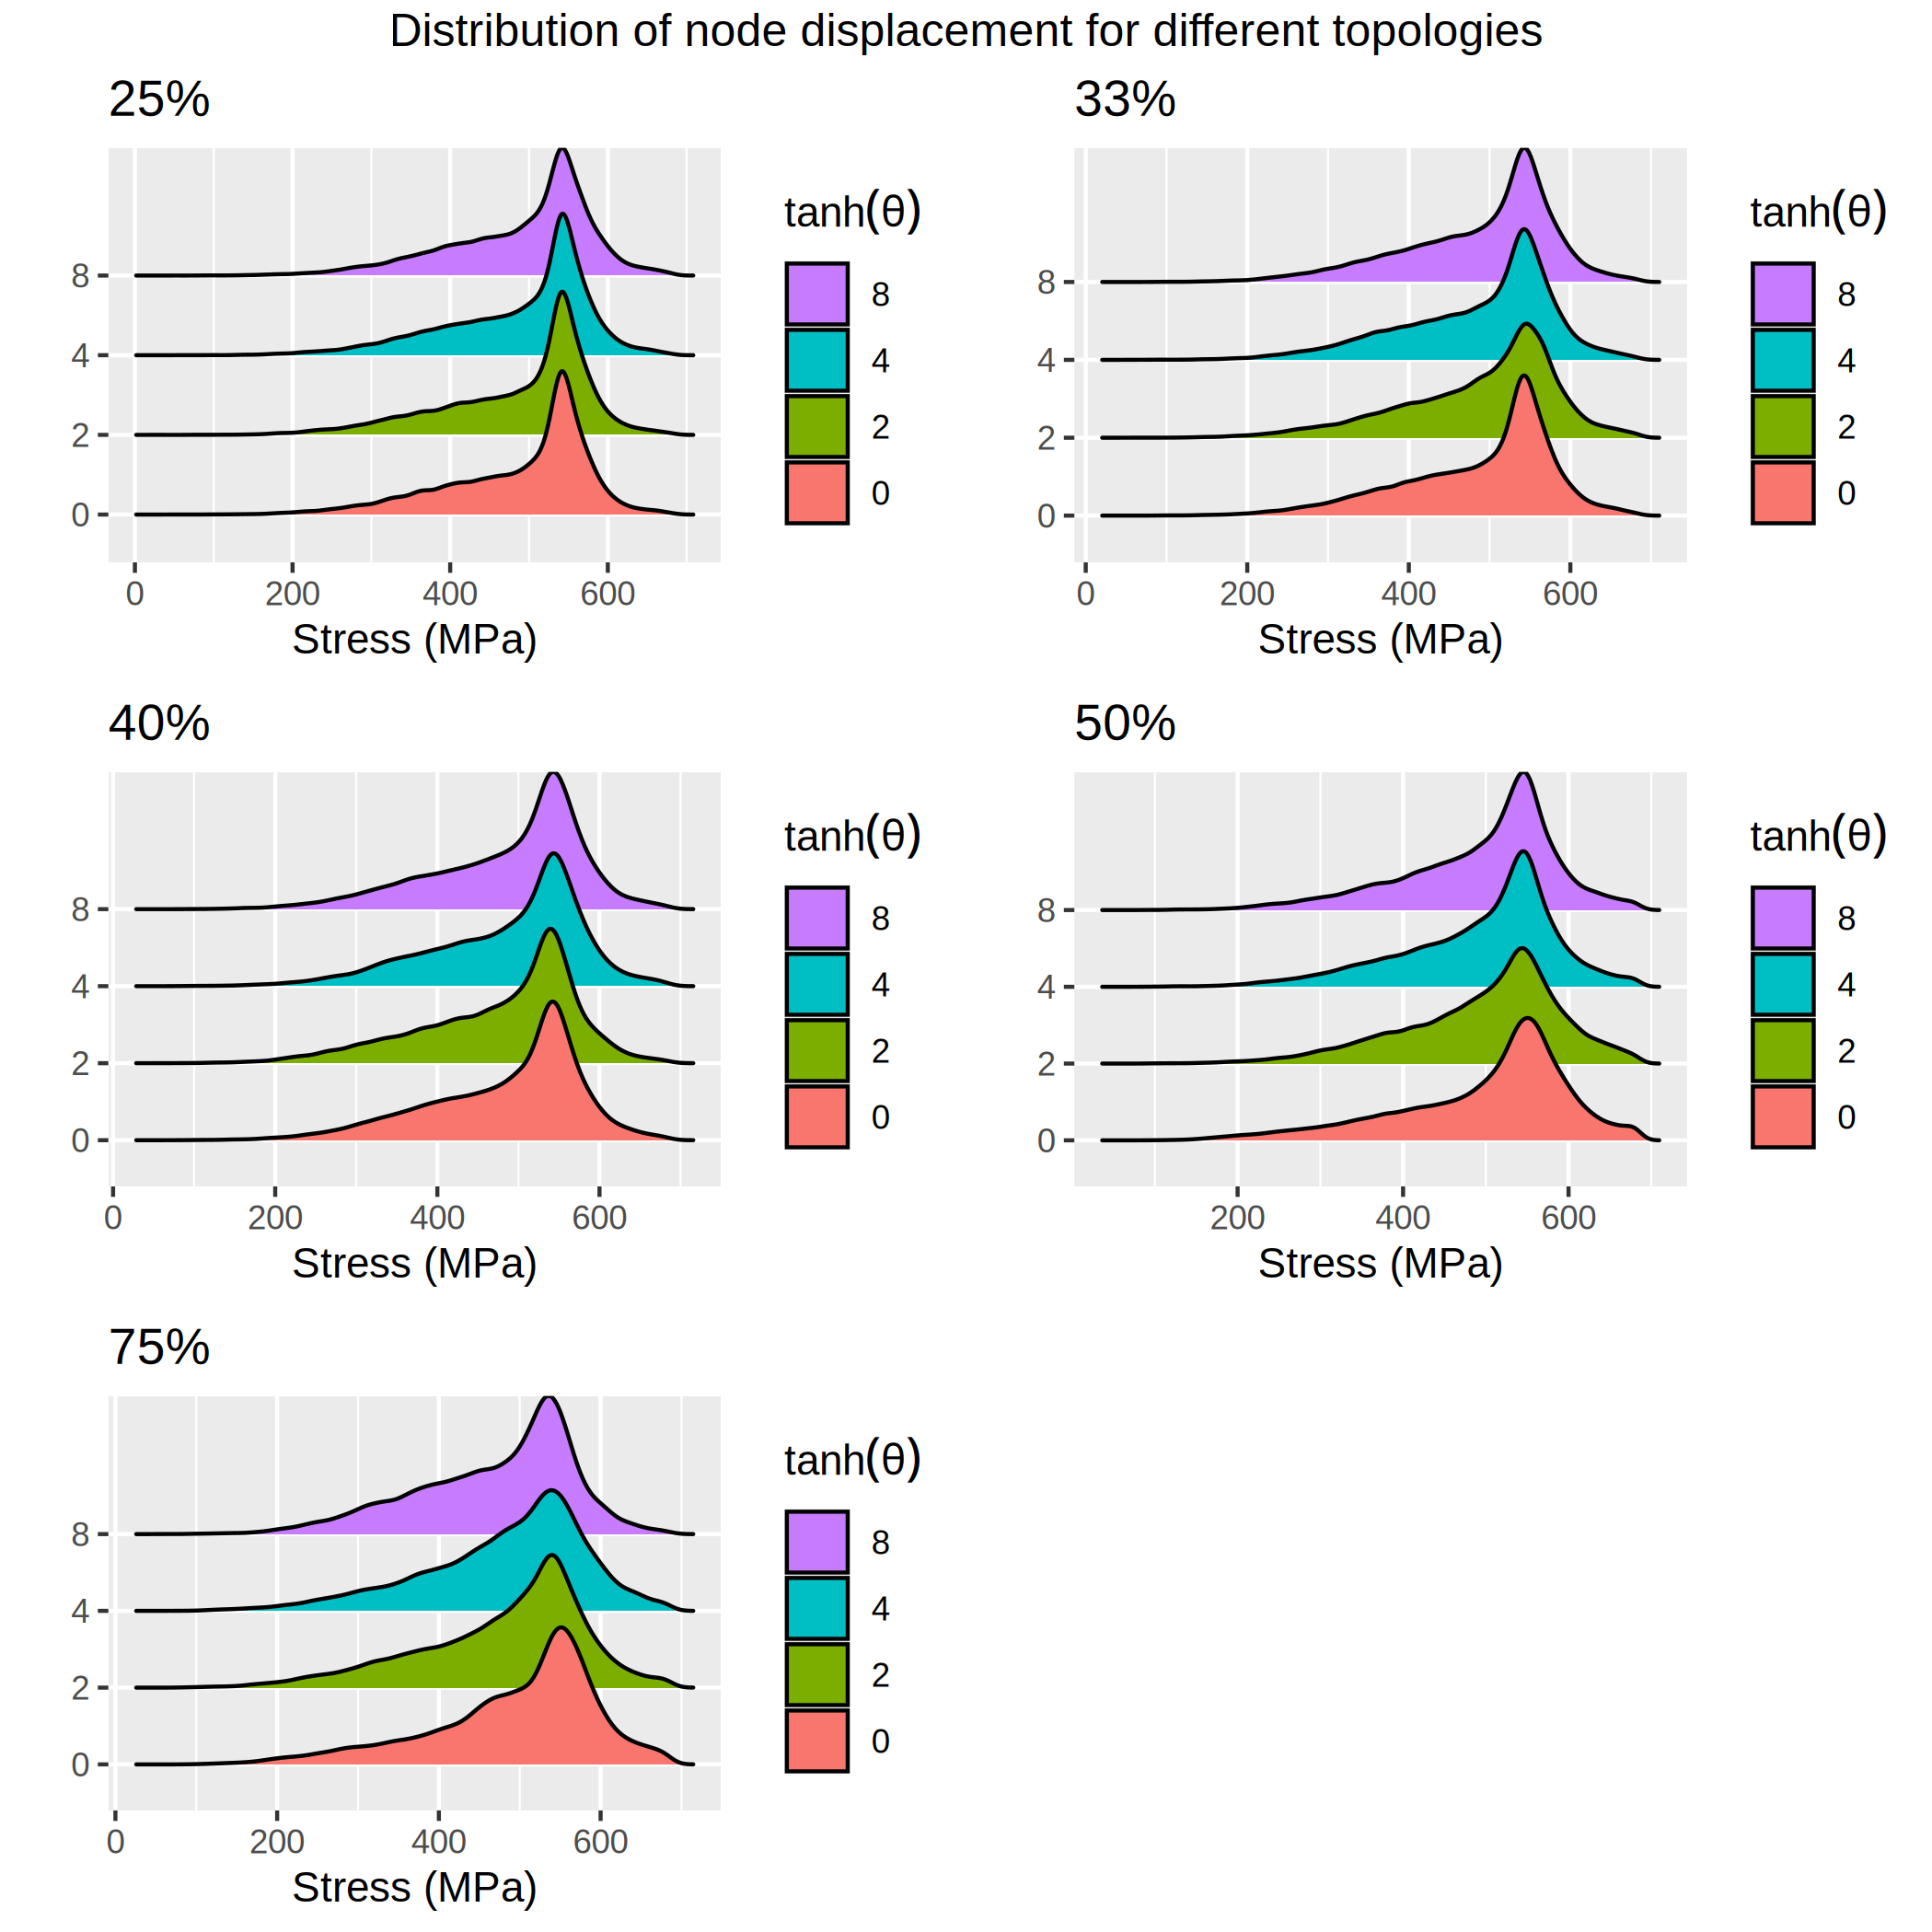
\includegraphics[width=0.75\textwidth]{images/results/plots/femoral/stress/stress_density_ridges.png}
\end{figure}

\begin{figure}[h!]
  \centering
  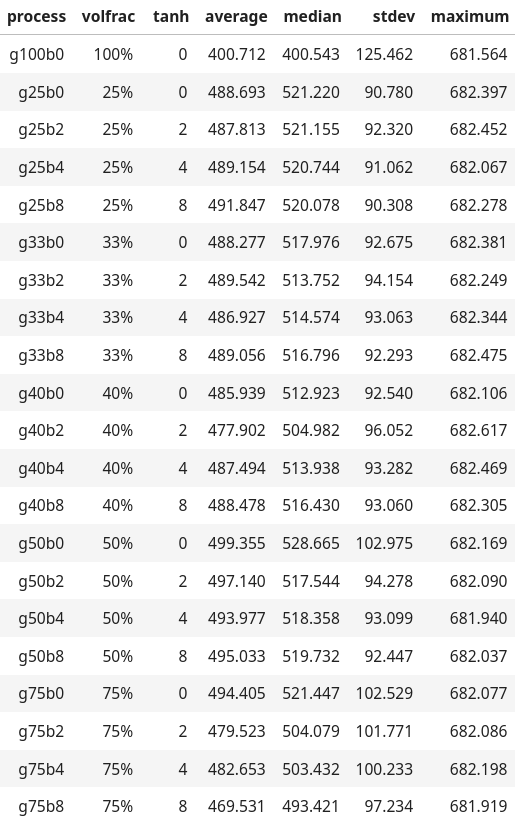
\includegraphics[width=0.75\textwidth]{images/results/plots/femoral/stress/stress_stats.png}
  \caption{Statistics of nodal stresses; all topologies}
  \label{fig:stress_stats}
\end{figure}

Next, we inspect the average deformation of the simulation results. We can see that the baseline case has the smallest average stresses, but as soon as topologies with lower volume fraction are used, the average stresses rises more than 20\%, from a baseline value of 400 MPa to over 485 MPa. The average stress does not change considerably from topology to topology, which is similar to what was noticed for the average nodal diplacement. Looking at the maximum stress yields a very interesting result; namely, that all of the topologies have a near constant maximum stress. This result is clear from looking at both graphs in Figure \ref{fig:maximum_stresses}.

\begin{figure}[h!]
  \centering
  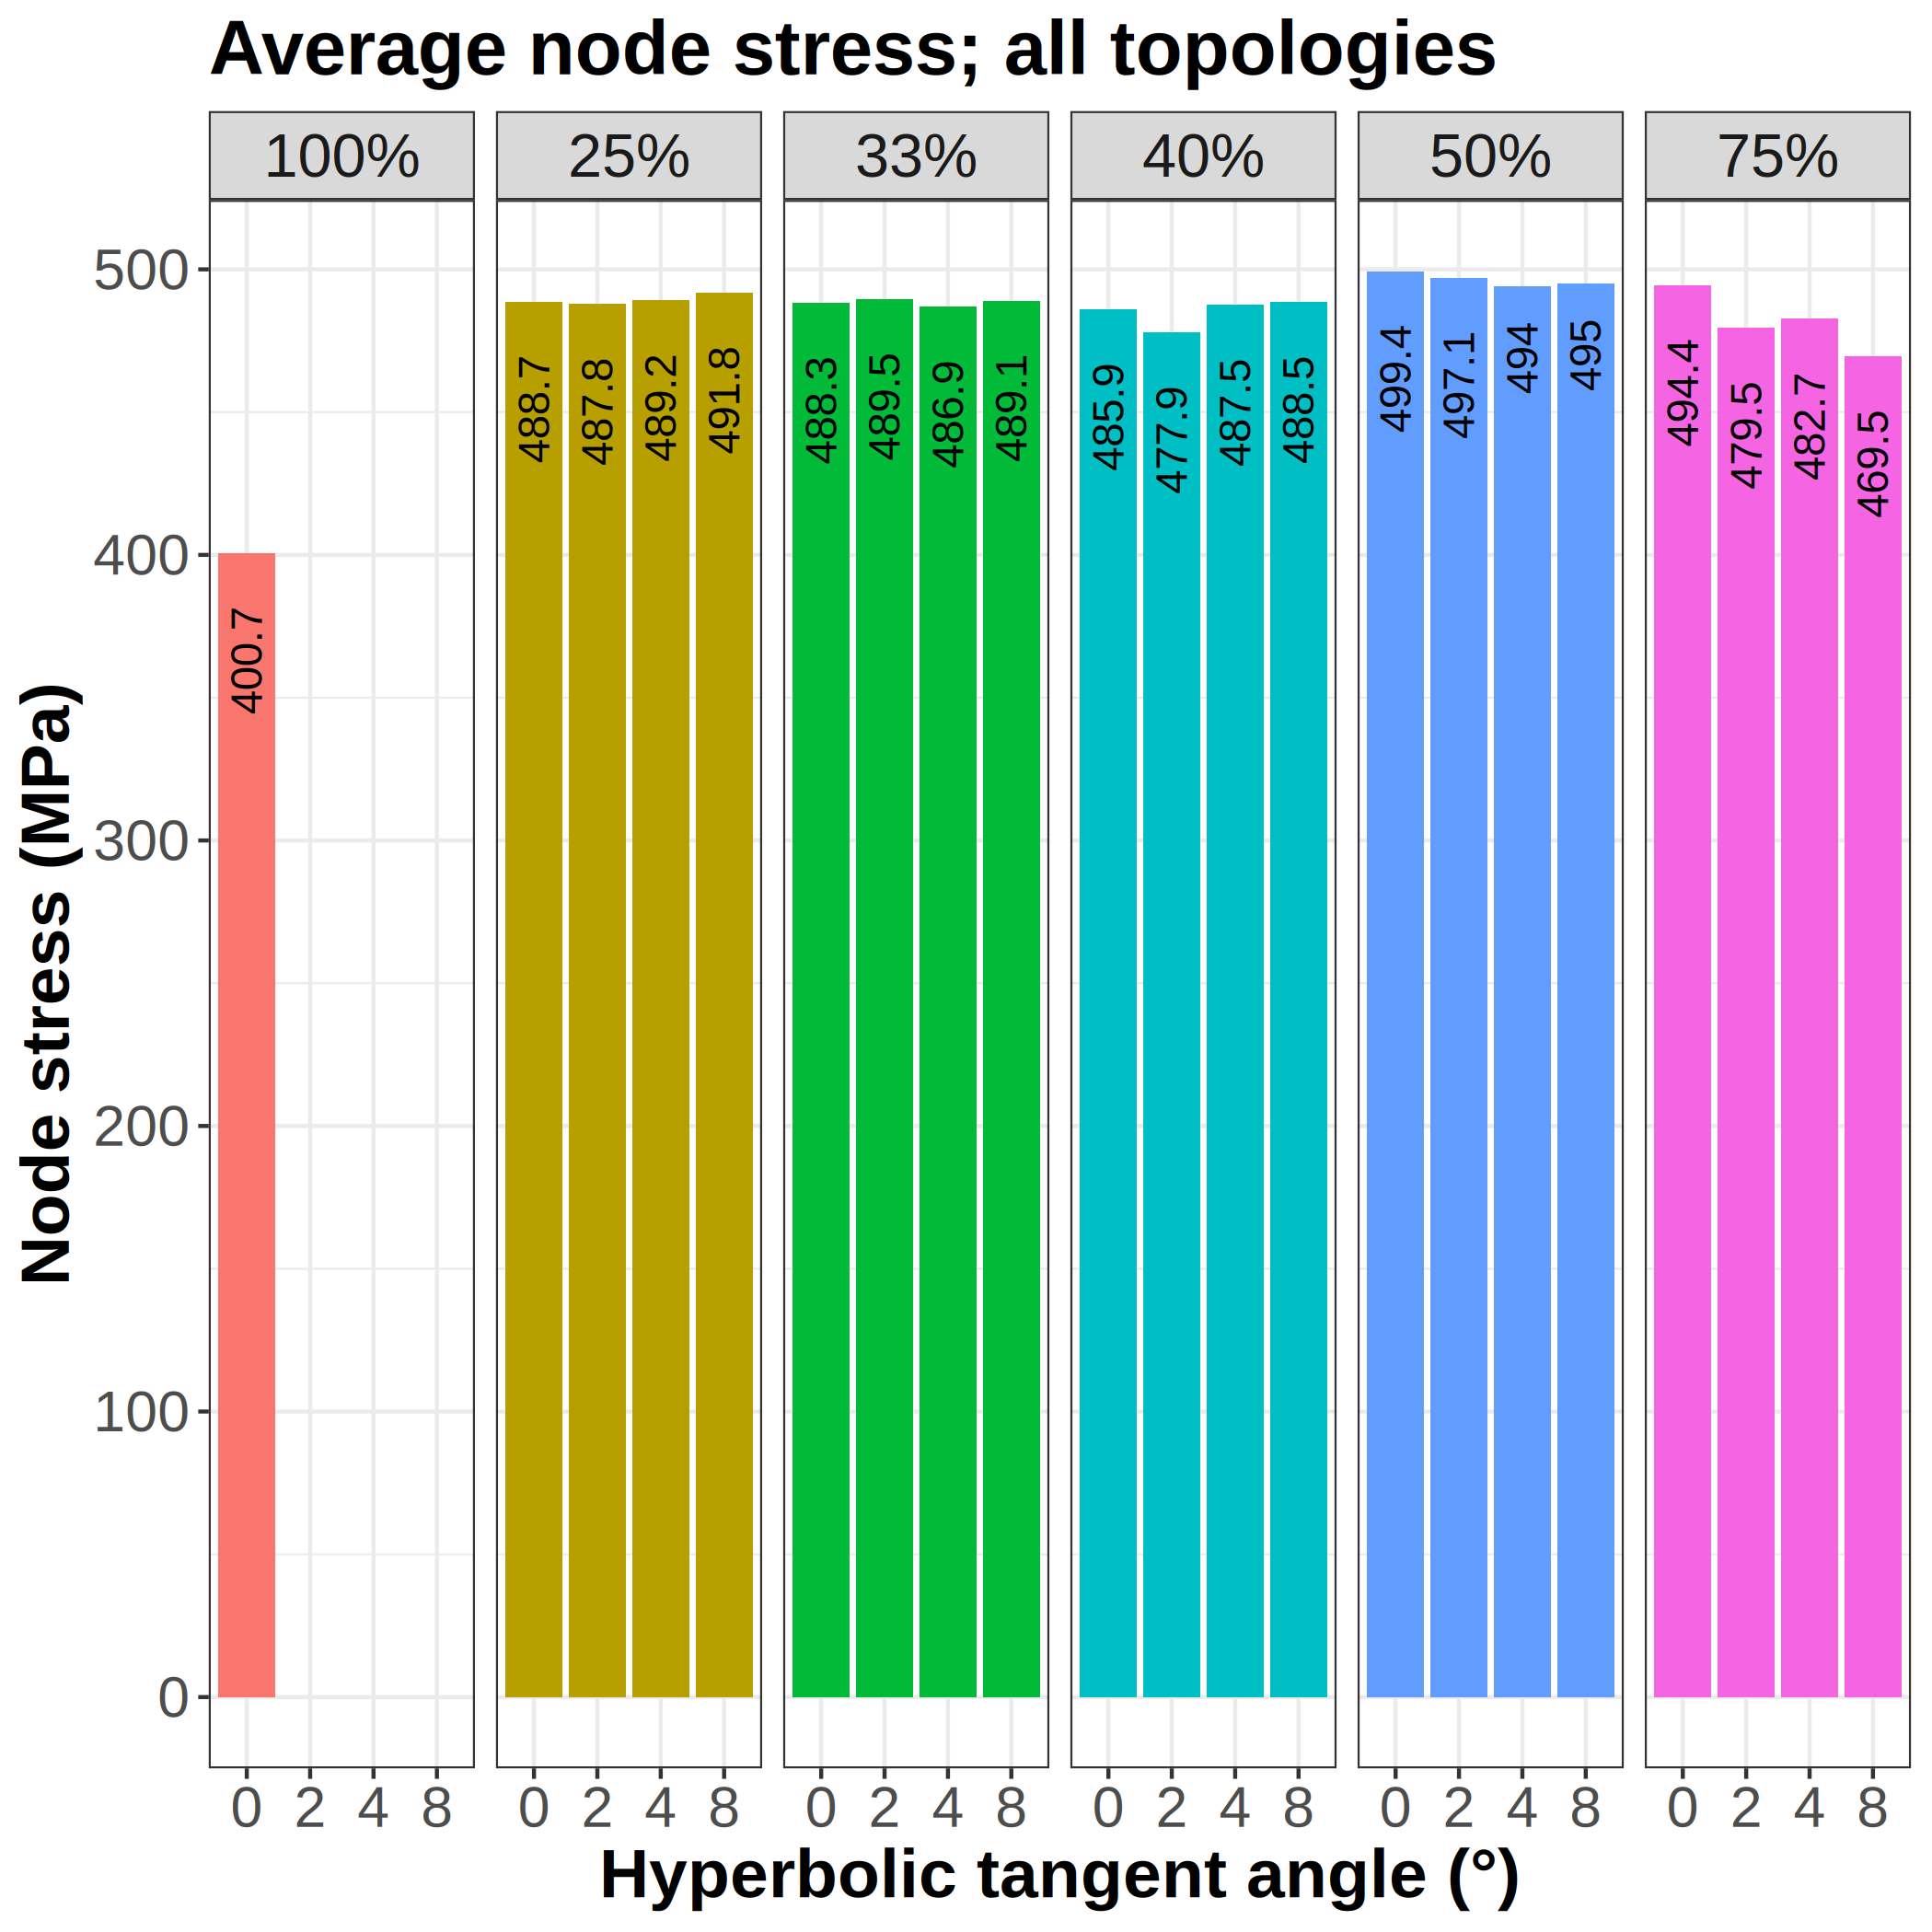
\includegraphics[width=0.45\textwidth]{images/results/plots/femoral/stress/average_stress.png}
  \hfill
  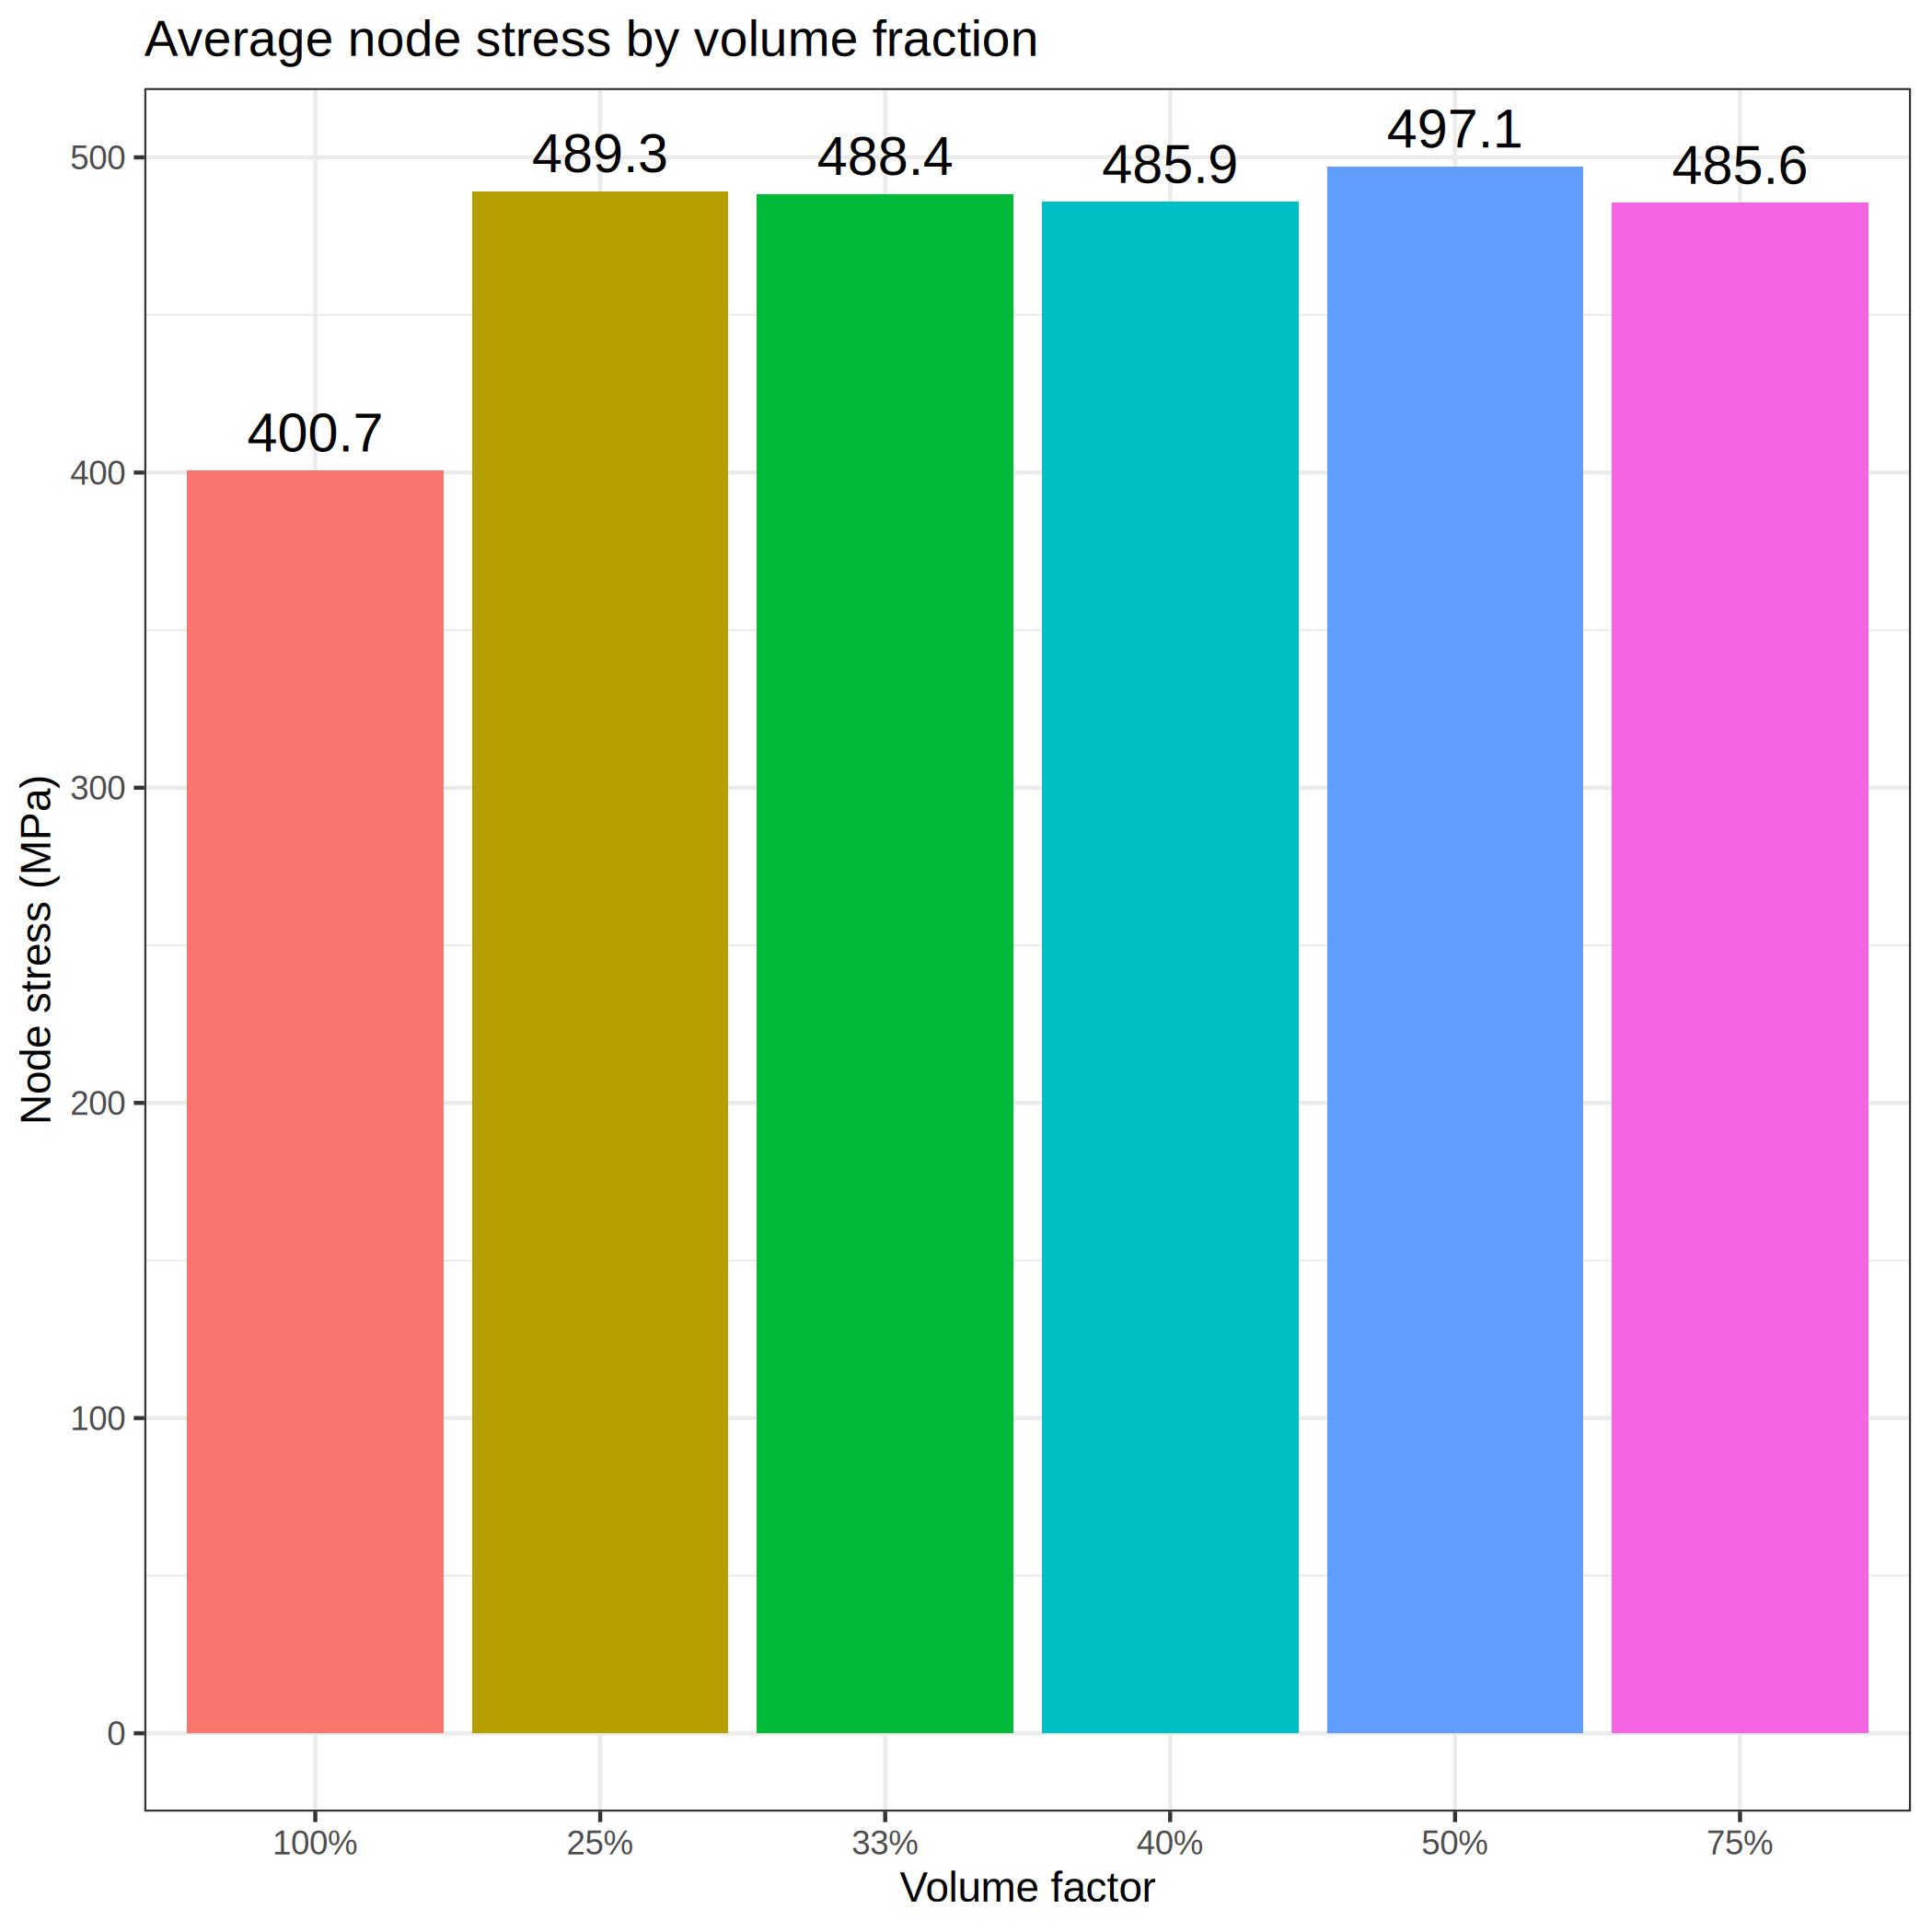
\includegraphics[width=0.45\textwidth]{images/results/plots/femoral/stress/femoral_average_group_stress.png}
  \caption{}
  \label{fig:average_stresses}
\end{figure}

\begin{figure}[h!]
  \centering
  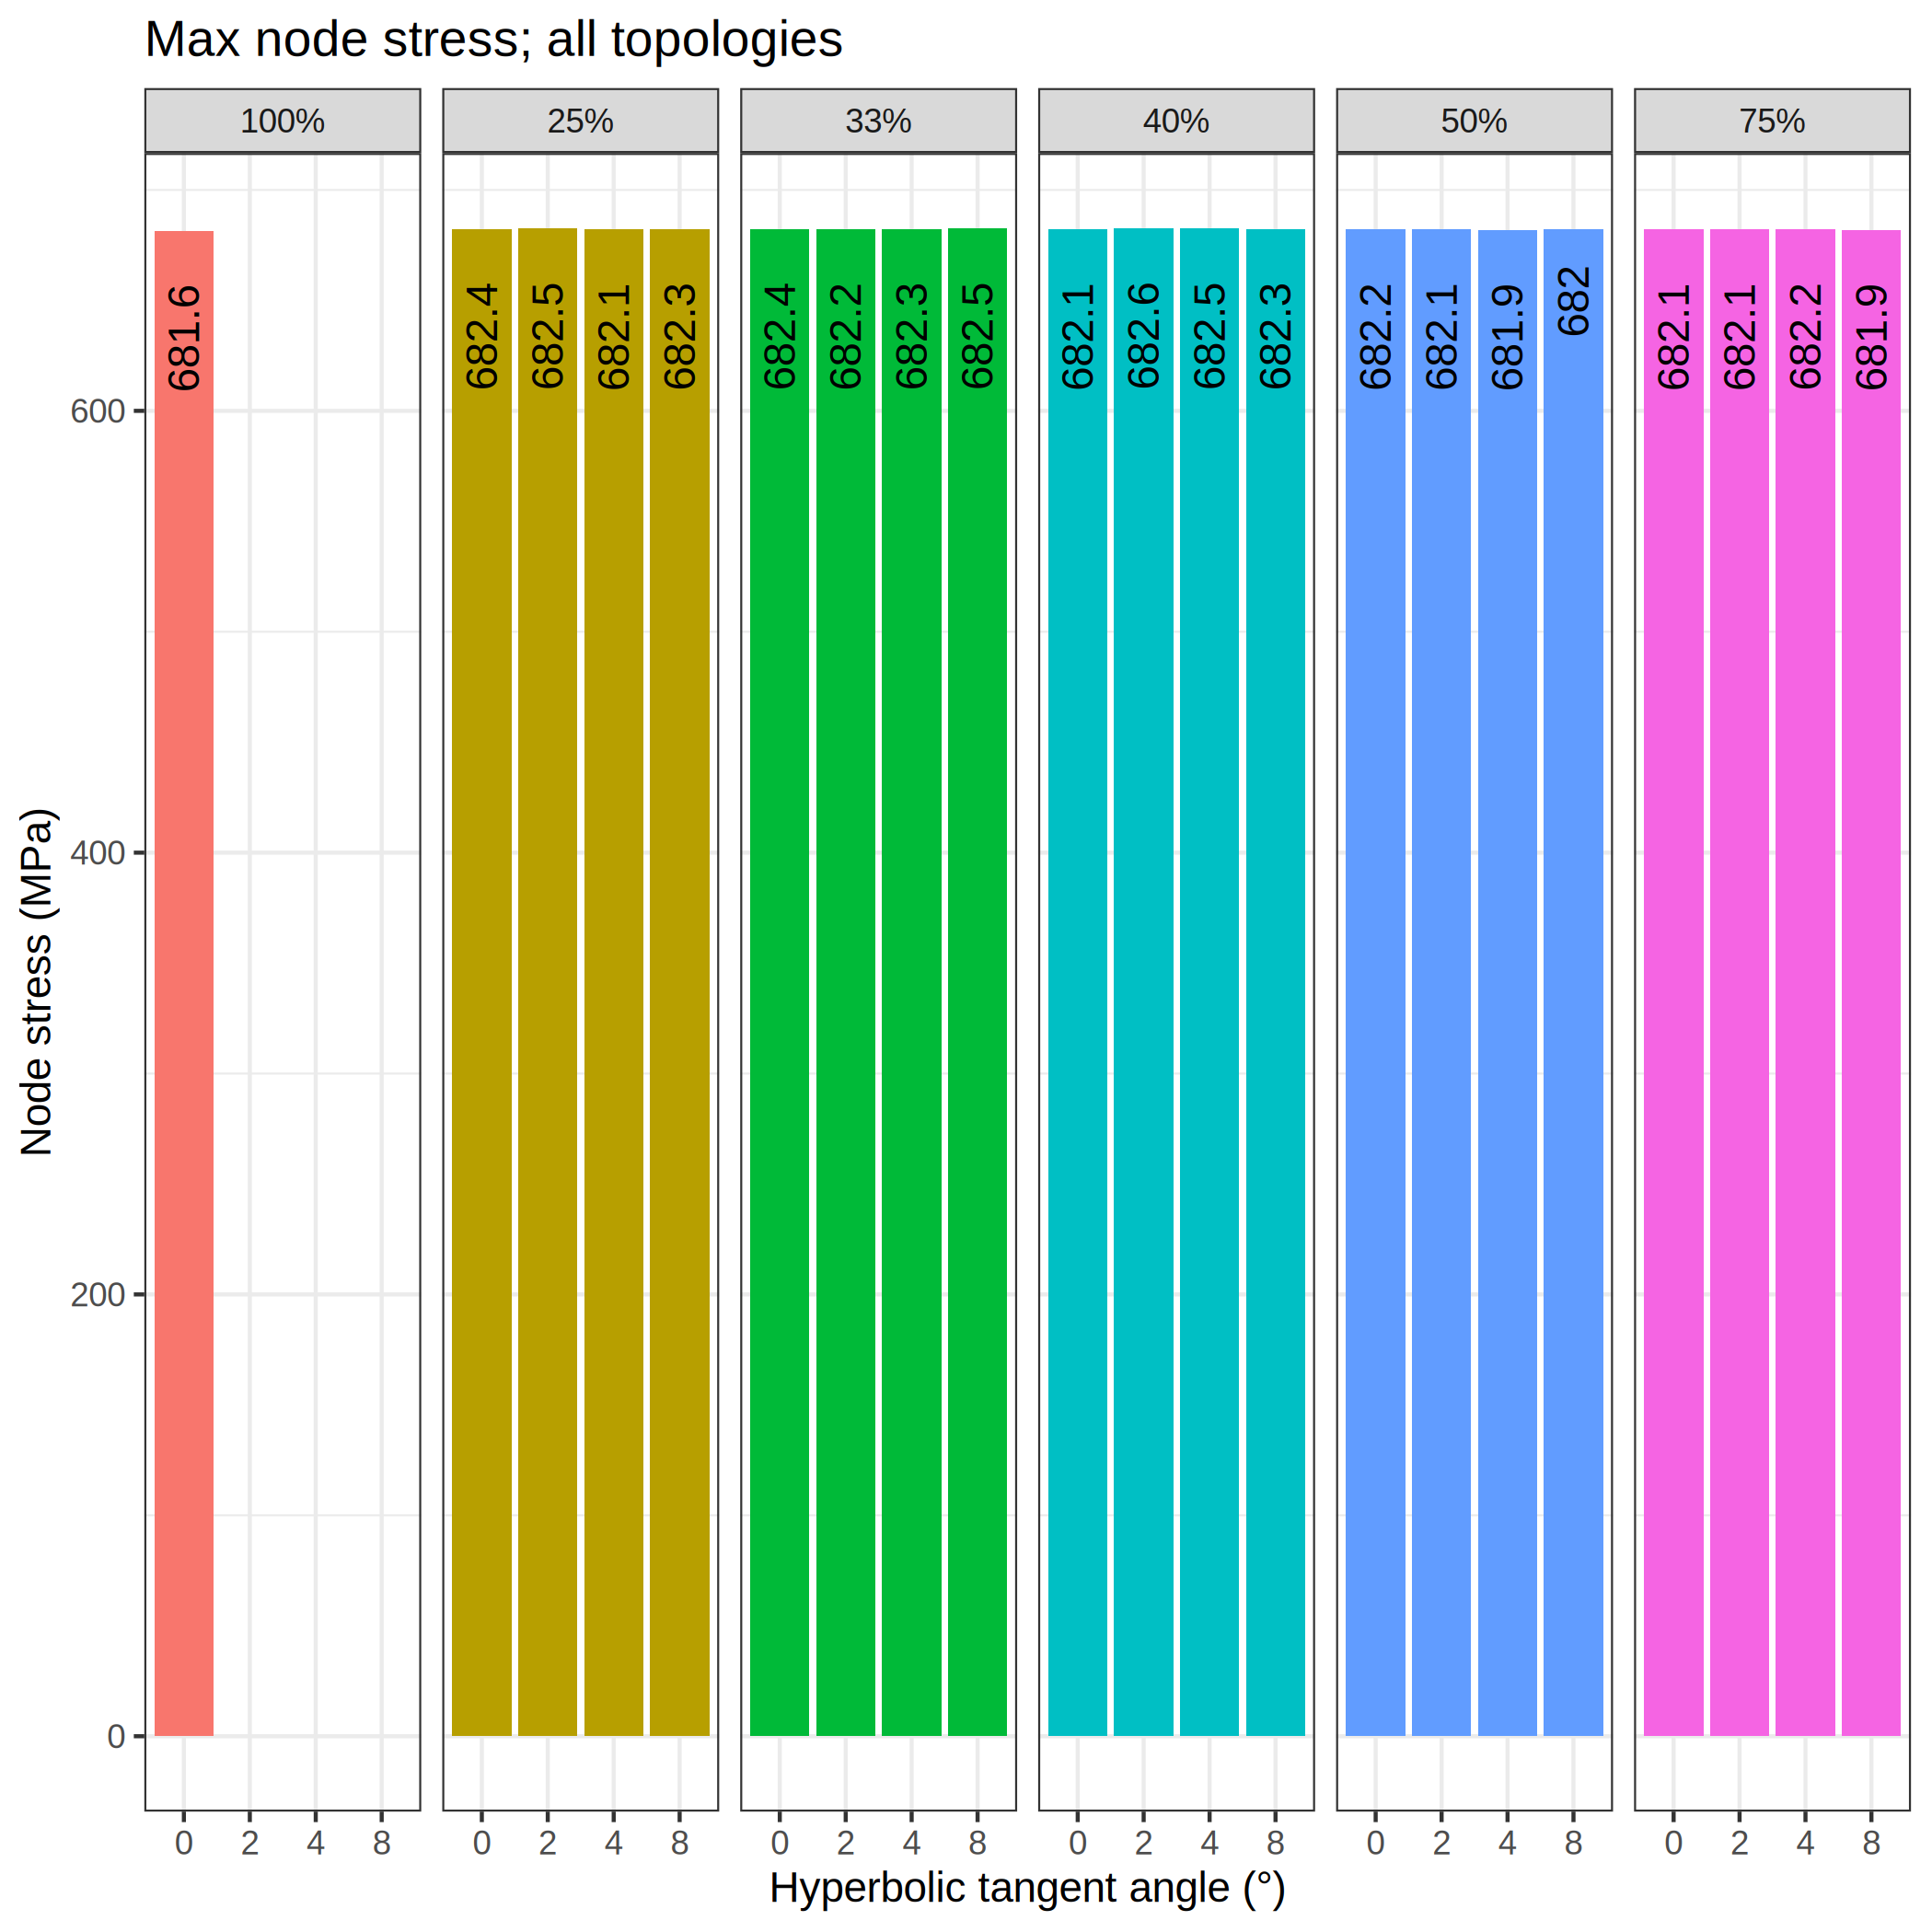
\includegraphics[width=0.45\textwidth]{images/results/plots/femoral/stress/maximum_stress.png}
  \hfill
  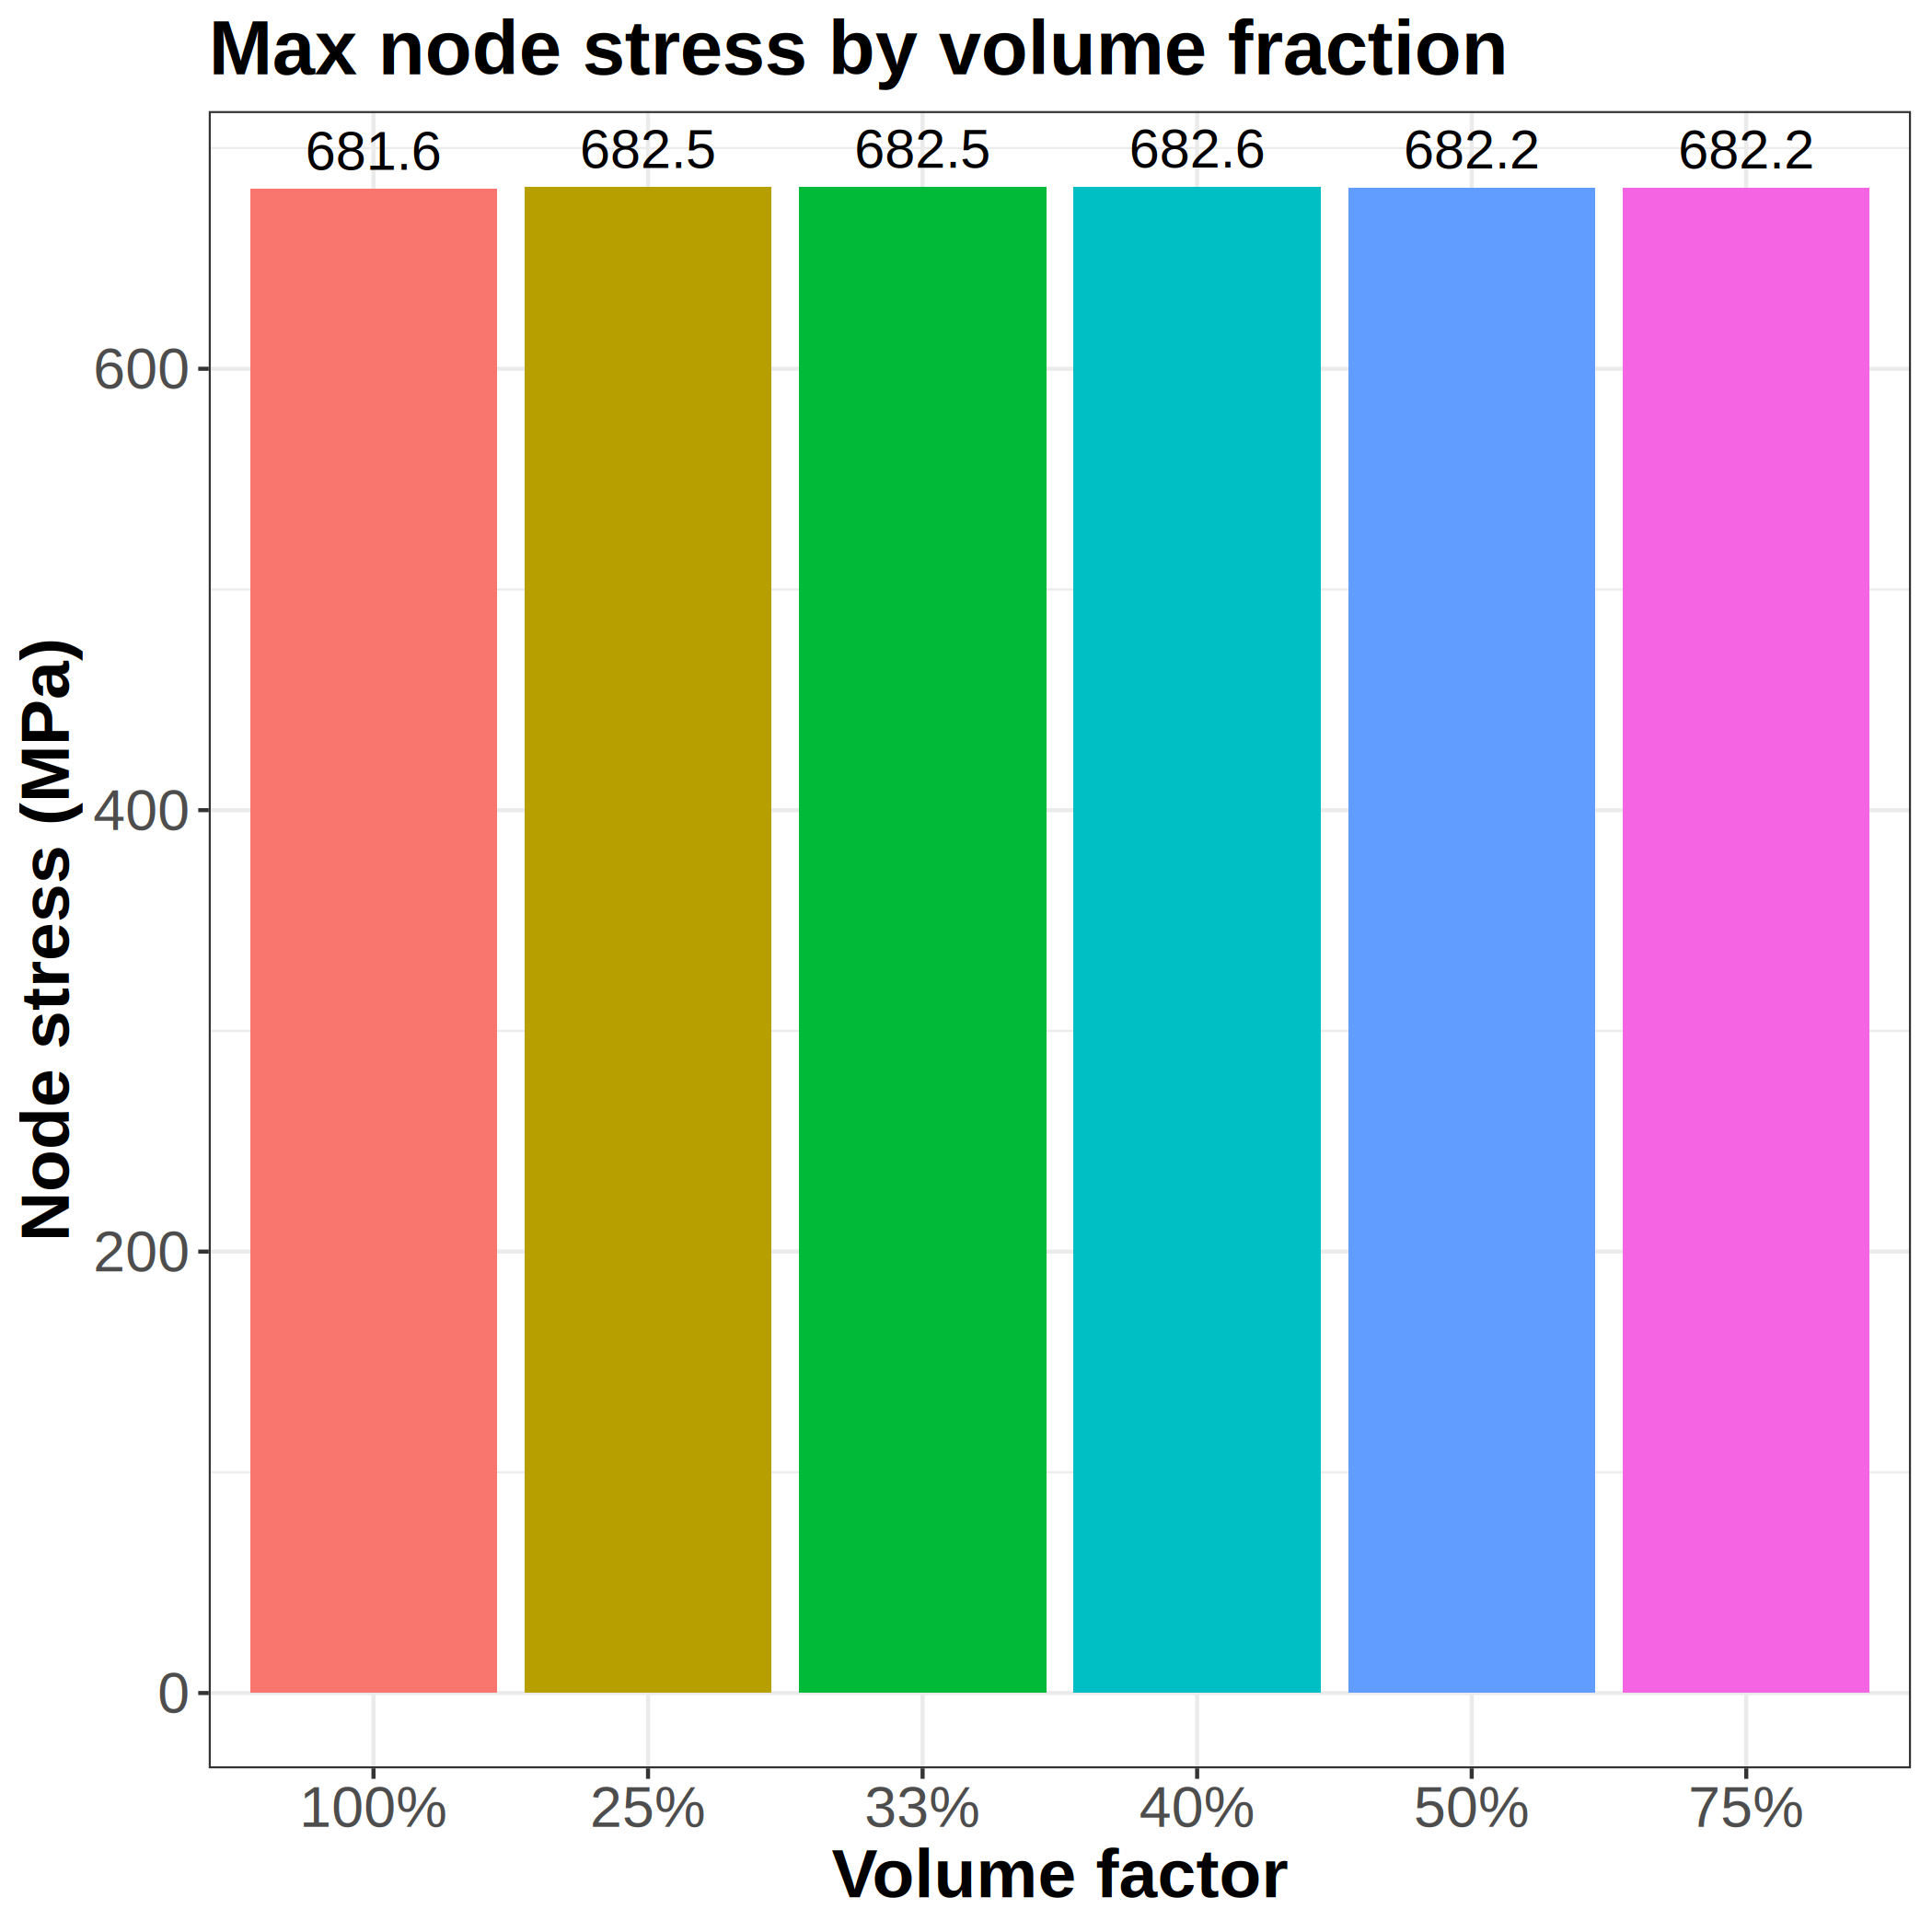
\includegraphics[width=0.45\textwidth]{images/results/plots/femoral/stress/femoral_max_group_stress.png}
  \caption{}
  \label{fig:maximum_stresses}
\end{figure}

Lastly, the box-whisker plot of Figure \ref{fig:stress_boxwhisker} shows a succint summary of all the statistics discussed in this section.

\begin{figure}[h!]
  \centering
  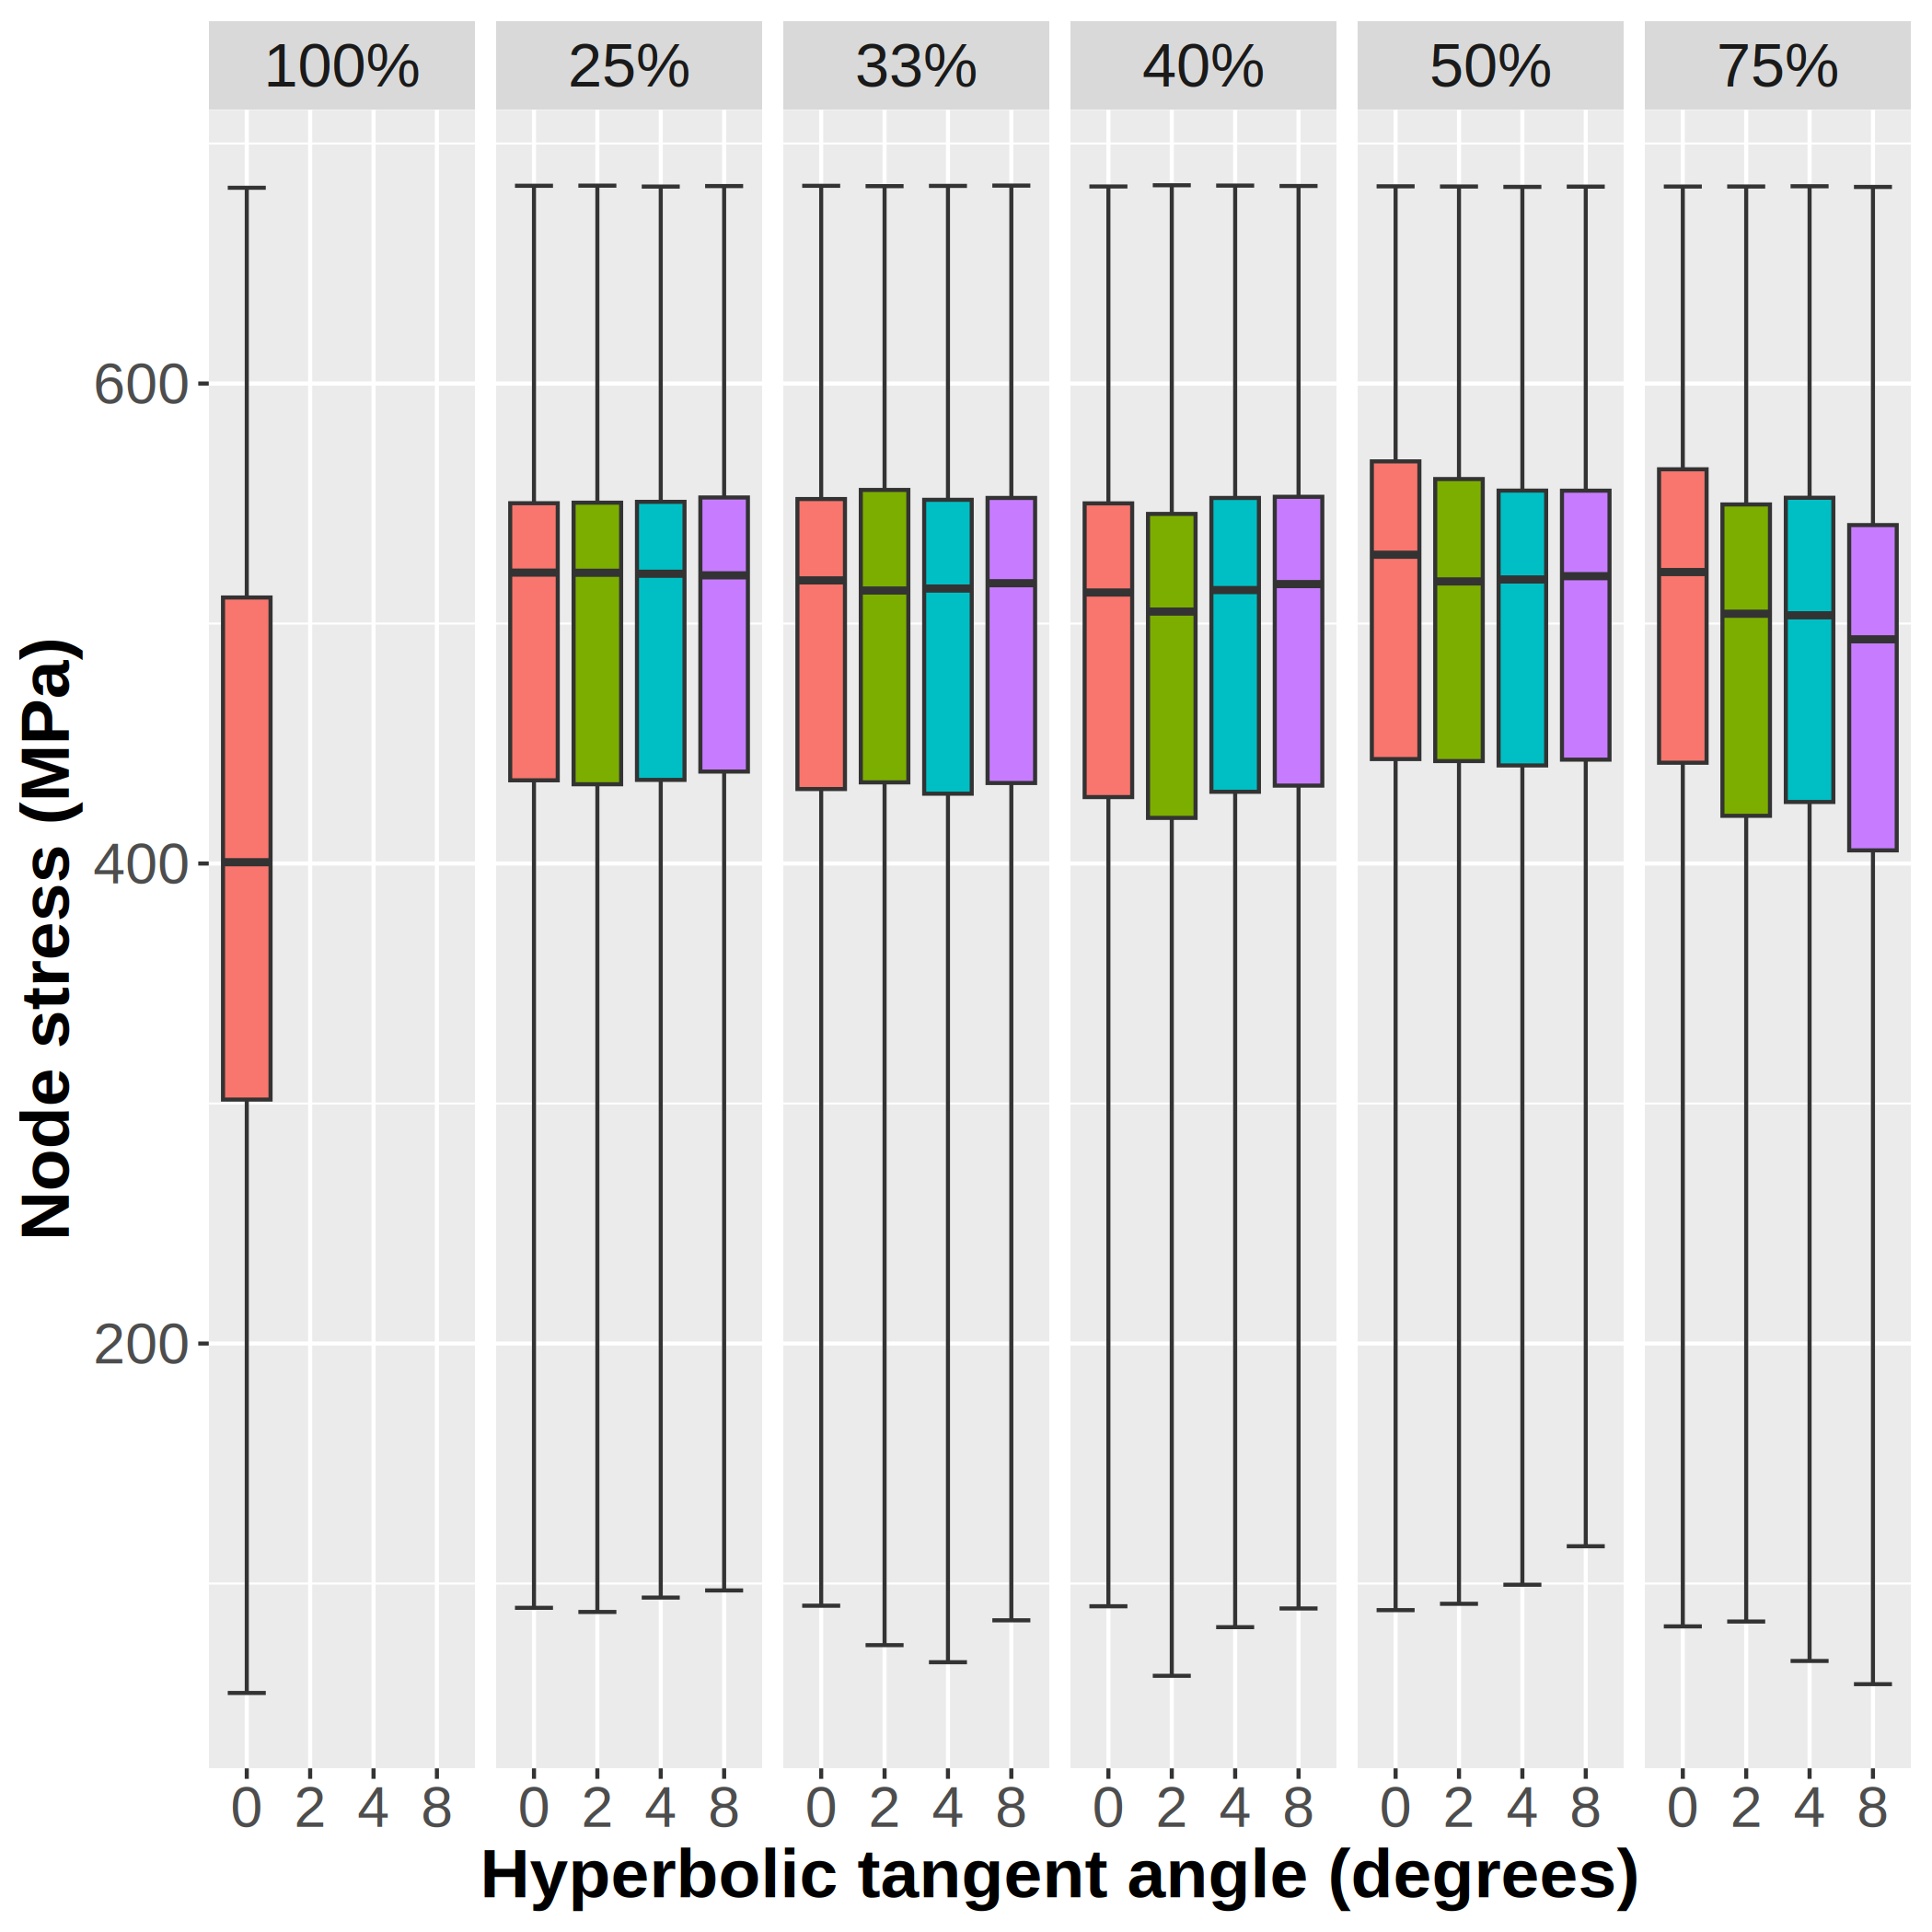
\includegraphics[width=0.8\textwidth]{images/results/plots/femoral/stress/boxplots.png}
  \caption{Box-and-whisker plot of nodal stress values of topologies of femoral component.}
  \label{fig:stress_boxwhisker}
\end{figure}


\end{document}
